% 2016 August
% LaTeX format and translation review by @fran2k, original translation by @fernando-sanz
% Formato en LaTeX y revisión de la traducción por @fran2k, traducción original por @fernando-sanz

\documentclass[a4paper,titlepage,final]{article}

\usepackage[utf8]{inputenc}
\usepackage{enumitem}
\usepackage{csquotes}
\usepackage{listings}
\usepackage{hyperref}
\usepackage{graphicx}
\setcounter{secnumdepth}{5}
\usepackage[a4paper,includeheadfoot,margin=2.54cm]{geometry}
\usepackage[spanish]{babel}

\begin{document}

\title{Steem\\* Una plataforma de social media con incentivos\\* basada en la blockchain}

\markboth{Steem Whitepaper}{Steem Whitepaper}

\author{Daniel Larimer, Ned Scott, Valentine Zavgorodnev, Benjamin Johnson,\\* James Calfee, Michael Vandeberg \\* \\* Traducción \href{https://steemit.com/@fernando-sanz}{@fernando-sanz}, Formato y revisión \href{https://steemit.com/@fran2k}{@fran2k}}

\date{Marzo 2016}

\begin{abstract}
Steem es una base de datos \textit{blockchain} que permite la contrucción comunitaria e interacción social con premios en criptomoneda. Steem combina conceptos de \textit{social media} con los aprendizajes provenientes de la construcción de criptomonedas y sus comunidades. Una clave importante para inspirar participación de cualquier comunidad, moneda o economía de libre mercado es un sistema de contabilidad justa que refleje consistentemente la contribución de cada persona. Steem es la primer criptomoneda que intenta recompenzar de forma acertada y transparente una cantidad indeterminada de individuos que realizan contribuciones subjetivas a su comunidad.
\end{abstract}

\maketitle

\tableofcontents

\newpage

\section{Introducción}

El contenido generado colectivamente por usuarios ha creado billones de dólares en valor para los accionista de compañias de \textit{social media} como Reddit, Facebook y Twitter. En 2014, Reddit hipotetizó que su plataforma podría ser mejorada si todos los que contribuyen en reddit.com posteando historias, agregando comentarios o votando fuesen premiados con una cantidad justa de participación en Reddit, Inc \cite{1}. Steem apunta a apoyar comunidades online y de \textit{social media} devolviendo gran parte de su valor a la gente que provee valiosas contribuciones, premiándolos con criptomoneda, y a través de este proceso crear una moneda que puede alcanzar un mercado masivo, incluyendo gente que aún no ha participado en alguna economía de criptomoneda.

Hay algunos principios clave que han sido utilizados para guiar el diseño de Steem. El más importante es que todos los que contribuyen a una empresa deben recibir una participación prorrateada, pago o débito de la empresa. Este principio es el mismo que se aplica en casi todas las \textit{Startups}, estas colocan acciones durante la fundación y durante rondas de inversión subsecuentes.

El segundo principio es que todas las formas de capital son igualmente valiosas. Esto significa que aquellos que contribuyen su escaso tiempo y atención en producir y curar contenido para otros, son tan valiosos como quienes contribuyen con su capital. Este es el principio de equidad de sudor\cite{2} y es un concepto que previo a las criptomonedas ha tenido problemas para proveer a no más de algunas docenas de individuos.

El tercer principio es que la comunidad produce productos para servir a sus miembors. Esto se ejemplifica con las uniones de crédito, coperativas de alimentos, planes de salud compartidos, que sirven a los miembros de sus comunidades mas que vender productos o servicios a la gente fuera de la comunidad.

La comunidad de Steem provee los siguientes servicios a sus miembros: 1. Una fuente de noticias y comentarios curada. 2. Medios para obtener respuestas de alta calidad a preguntas personalizadas. 3. Una criptomoneda estable vinculada al Dólar Estadounidense. 4. Pagos libres. 5. Trabajos que proveen los servicios antes mencionados a otros miembros.

El útil realineamiento de incentivos económicos de Steem tiene el potencial de producir resultados justos y mas inclusivos para todos los involucrados que las plataformas de \textit{social media} y criptomonedas que la preceden.

Este documento explorará los incentivos económicos existentes y demostrará cómo Steem y sus incentivos podrán resultar mejor para la mayoría de los participantes.

\subsection{Reconociendo las contribuciones}
Steem está diseñado desde cero para resolver las mayores barreras para su adopción y monetizaciones de una economías basada en \textit{social media}. Nuestra tésis es que las mismas técnicas usadas para hacer crecer las mas grandes plataformas de \textit{social media} pueden ser utilizadas para iniciar una criptomoneda existosa. Incentivos económicos habilitados por criptomoneda pueden facilitar dramáticamente el crecimientod de una nueva plataforma de \textit{social media}. Es la sinergía entre criptomoneda y \textit{social media} lo que creemos que puede dar a Steem una poderosa ventaja en el mercado.

El reto afrontado por Steem es derivar un algoritmo para tasar contribuciones individuales que la mayor parte de los miembros de la comunidad consideren una evaluación justa del valor subjetivo de cada contribución. En un mundo perfecto, los miembros de la comunidad coperarían para valuar la contribución de cada par y devolver una justa compensación. En el mundo real, deben diseñarse algoritmos de tal forma que sean resistentes a manipulación intencional con fines de lucro. Cualquier abuso del sistema de tasación podría causar la pérdida de fe en la percepción de justicia del sistema económico por parte de sus miembros.

Las plataformas existentes operan en un principio de un usuario, un voto. Esto crea un ambiente donde los rankings pueden ser manipulados por ataques de profeta y los proveedores de servicio deben proactivamente identificar y bloquar abusadores. La gente actualmente intenta manipular los sistemas de tasacipon de Reddit, Twitter y Facebook siendo la única ganancia el tráfico web o la censura.

La unidad fundamental de contabilidad en la plataforma de Steem es STEEM, un token de criptomoneda. Steem opera en la base de un STEEM, un voto. Bajo este modelo, los individuos que mas hayan contribuido a la plataforma, segun lo corroborado por el balance de su cuenta, tienen mayor influencia sobre cómo se valúan las contribuciones. Además, Steem solo permite a los miembros votar con STEEM cuando este es sujeto a un esquema multi-anual de adquisición. Los miembros tienen un incentivo financiero para votar en el sentido que ésto maximiza el valor a largo plazo de sus propios STEEM.

Steem está diseñado alrededor de un concepto relativamente simple: toda contribución significativa a la comunidad debería ser reconocida por el valor que añade. Cuando la gente es reconocida por sus contribuciones, continúan contribuyendo y la comunidad crece. Cualquier desbalance en el ida y vuelta dentro de una comunidad es insustentable. Eventualmente los dadores se cansan de soportar a los miembros que restan y atentan contra la comunidad.

El reto es crear un sistema capaz de identificar qué contribuciones son necesarias y su valor relativo de manera que pueda escalar a un numero indeterminado de gente. Un sistema comprobado para evaluar y premiar contribuciones es el libre mercado. El libre mercado puede ser visto como una comunidad única donde todos intercambian con otros y las recompenzas son asignadas por pérdidas y ganancias. El sistema de mercado premia aquellos que proveen valor a otros y castiga a quienes consumen más valor del que producen. El mercado libre soporta muchas monedas diferentes y el dinero es simplemente una \textit{commodity} que todos encuentran fácil de intercambiar.

Desde que el libre mercado es un sistema comprobado, es tentador intentar crear un sistema de igual característica donde los consumidores de contenido pagan directamente a los productores del mismo. De todas formas, el pago directo es ineficiente y realmente inviable para la creación y curado de contenido. El valor de la mayoría del contenido es muy bajo en relación con el costo cognitivo, financiero y de oportunidad asociado con hacer un pago que algunos pocos lectores eligen beneficiar. La abundancia de alternativas libres siginifica que la aplicación de un \textit{paywall} derivará a los lectores a otro lado. Han habido gran cantidad de intentos de implementar micro pagos por artículo de parte de los lectores hacia los autores, pero ninguno se ha alcanzado una amplitud considerable.

Steem está diseñado para permitir micropagos efectivos por cualquier tipo de contribución al cambiar la ecuación económica. Los lectores ya no tienen que decidir si pagar o no a alguien desde su propio bolsillo, en cambio votan o restan votos y Steem usa estos votos para determinar premios individuales. Esto significa que se le otorga a la gente una interfaz familiar y ampliamente utilizada y ya no enfrentan los costos de oportunidad, cognitivos y financieros asociados tradicionalmente a los micropagos y plataformas de propinas.

El voto de los miembros de la comunidad es crítico para que Steem acomode los pagos a los contribuyentes de forma precisa. El voto puede por lo tanto ser visto como una contribución crucial y digno de ser recompenzado en sí mismo. Algunas plataformas, como Slashdot, usan meta-moderación\cite{3} como una forma de rankear y premiar a los moderadores honestos. Steem entonces premia a quienes mas contribuyen al total de la promoción de una pieza de contenido pagando a los votantes proporcionalmente al pago principal del creador del contenido votado.

Hay otras formas de contribución que Steem reconoce y premia usando métricas objetivas. Entre ellas están: validación de transacciones, minado de prueba de trabajo, premios de liquidez, y reportado de productores de bloque malitencionados.

\section{Formas de contribuir}

Esta sección delínea las ideas detrás de Steem y sus recompenzas para la gente que provee contribuciones significativas y mesurables a la comunidad de Steem.

\subsection{Contribuciones de capital}

Hay dos items que una comunidad puede ofrecer para atraer capital: deuda y propiedad. Quienes compran propiedad ganan cuando la comunidad crece pero pierden si la misma decrece. Quienes compran deuda obtienen la garantia de un cierto monto de interpes pero no llegan a participar de las ganancias realizadas por el crecimiento de la comunidad. Ambos tipos de contribuciones de capital son valiosas para el crecimiento de la comunidad y la valuación de su moneda. Adicionalmente hay dos formas en que la propiedad puede conservarse: liquidez y colocación. La colocación de propiedad genera un compromiso de largo plazo y no puede ser vendida por un determinado período de tiempo.

La red Steem denomina a estas diferentes clases de assets Steem (STEEM), Steem Power (SP), y \textit{Steem Dollars} (SMD)

\subsection{Steem (STEEM)}

Steem es la unidad fundamental contable en el \textit{blockchain} de Steem. Los demás tokes derivan su valor del de STEEM. Generalmente STEEM deberia ser mantenido por cortos períodos de tiempo cuando se necesita liquidez. Alguien que busque entrar o salir de la plataforma de Steem tendrá que comprar o vender STEEM. Una vez comprado debería ser convertido a SP o SMD para mitigar el impacto de la dilución en el largo plazo. STEEM crece constantemente en oferta por un 100\% anual debido a incentivos no SMD. Quien tenga STEEM sin convertirlos a SP, se diluirán aproximadamente en un 0.19\% diario. Mientras el ritmo puede parecer alto, para transacciones que toman menos de 10 dias, sigue siendo mas barato que las comisiones de proceso de tarjetas de crédito. Ademas, la creación diaria de \textit{tokens} es insignificante al lado de la volatilidad diaria.

Quien compre \textit{Bitcoin} o cualquier otra criptomoneda y la venda 10 dias después podría perder fácilmente 3\% o mas debido a las fluctuaciones de precio. Quien compre \textit{Bitcoin} y luego lo venda en el mismo dia usualmente pagará mas del 0.4\% sólo en comisiones del mercado de intercambio. En otras palabras, el ritmo de inflacipon es efectivamente insignificante durante el período de tiempo que un individuo típico sostendrá STEEM.

La mayoría de la inflación es de hecho un artefacto de contabilidad en lugar de un verdadero reacomodamiento de riqueza. El 90\% de la inflación no SMD es redistribuída a los poseedores existentes de STEEM proporcionalmente al valor de STEEM de su balance de SP, convirtiendo la inflación en mas bien una repartición. Solo alrrededor del 10\% de la inflación no SMD redistribuye propiedad en la red.

\subsection{Steem Power (SP)}

Las \textit{Startups} o los emprendimientos requieren un compromiso de capital a largo plazo. Aquellos que invierten su dinero en estas companías calculan esperar años antes de poder vender sus acciones y efectivizar su ganancia. Sin compromiso a largo plazo, una startup buscando recolectar capital adicionar a través de la venta de acciones adicionales estaría compitiendo con accionistas existentes queriendo retirarse. Los inversores compresivos quieren que sus contribuciones de capital hagan crecer la compañía, pero el crecimiento no puede suceder si el nuevo capital es entregado a los que buscan retirarse.

Hay un valor significativo en tener compromiso a largo plazo porque habilita a las comunidades a hacer planes a largo plazo. El compromiso a largo plazo de los accionistas también causa que estos voten por el crecimiento a largo plazo en lugar de bombeos de corto plazo.

En el espacio de las criptomonedas, los especuladores saltan de criptomoneda en criptomoneda basados mayormente en las expectativas de crecimiento a corto plazo. Steem busca armar una comunidad que sea propiedad y controlada enteramente por aquellos con perspectivas a largo plazo. Debido a que Steem busca alentar el crecimiento a largo plazo, está fijado en su lógica la acomodación de 9 STEEM a los poseedores de Steem Power (SP) por cada STEEM que crea para financiar el crecimiento a través de incentivos a la contribución. En el tiempo, esto lleva a que la relación entre el total de valor en STEEM de Steem Power (SP) se balacee al total de los balances STEEM hacia un 9:1. (Al parecer, esta relación probablemente supere el 9:1 debido al contínuo empoderamiento de la red de los nuevos STEEM emitidos) Esto también significa que los poseedores a largo plazo son protegidos casi por completo de la dilución utilizada en la financiación del crecimiento.

Los SP sólo pueden ser convertidos a STEEM luego de 2 años a través de 104 pagos semanales equitativos. 1 SP puede ser visto como una acción en un pool de STEEM. La red automáticamente agrega STEEM al pool en cada bloque. En cualquier momento, los usuarios pueden convertir sus STEEM en SP en la misma relación en que el STEEM en el pool de plazos fijos al total de SP. Convertir STEEM a SP no diluye a los poseedores existentes de SP. Mas bien, cada vez que se convierte de SP a STEEM, se hace con la relación del momento. Los individuos tienen garantizado poseer mas STEEM en el futuro de lo que tienen cuando convierten por primera vez desde STEEM a SP.

Los balances de SP son no-transferibles y no-divisibles excepto a través de las solicitudes recurrentes automáticas de conversión. Esto significa que el SP no puede ser intercambiado en \textit{exchanges} de criptomonedas.

Poseer SP es requerido para votar a favor o denunciar contenido. Esto quiere decir que el SP es el token de acceso que otorga a sus poseedores poderes exclusivos dentro de la plataforma de Steem.

La acción de transferir desde STEEM a SP es llamada \textit{Powering Up} mientras que la transferencia de SP a STEEM es \textit{Powering Down}. Por ejemplo, uno puede hacer \textit{Power Down} de sus STEEM sobre un período de 2 años, pero se puede hacer \textit{Power Up} con sus STEEM inmediatamente.

\subsection{\textit{Steem Dollars} (SMD)}

La estabilidad es un componente importante en las economías globales exitosas. Sin estabilidad, los individuos en distintas partes del mundo no podrían tener costos cognitivos bajos al participar en el comercio y ahorro. Por este motivo, los \textit{Steem Dollars} fueron diseñados como un intento de traer estabilidad al mundo de las criptomonedas y a los individuos que usen la red Steem.

Los \textit{Steem Dollars} (SMD) son creados por un mecanismo similar a las notas convertibles, que son usualmente utilizadas para financias \textit{Startups}. En el mundo de las \textit{Startups}, las notas convertibles son instrumentos de deuda a corto plazo que pueden ser convertidos a propiedad a un ritmo determinado en el futuro, típicamente durante una futura ronda de inversión. Un token basado en \textit{blockchain} puede ser visto como propiedad mientras una nota convertible puede ser vista como deuda con denominación en otra \textit{commodity} o moneda. Los términos de la nota convertible permiten a su dueño convertirla al token que la respalda con una antelación mínima al precio justo del mercado del token. Crear dólares convertibles a \textit{tokens} habilita a los \textit{blockchains} a aumentar su efecto de red mientras se maximiza el retorno a los poseedores de \textit{tokens}.

Los \textit{Steem Dollars} son nomenclados con el símbolo SMD, su acrónimo. Para crear los SMD se requiere una combinación entre un indicador de precio confiable, reglas para prevenir el abuso, y liquidez. Proveer un indicador de precio confiable implica tres factores: minimizar el impacto de un indicador incorrecto, maximizar el costo de producir un indicador incorrecto, y minimazar la importancia de la cadencia.

\subsubsection{Minimizando comisiones fraudulentas}

Los poseedores de SP eligen individuos para publicar indicadores de precio. Estos individuos seleccionados son presumiblemente poseen la confianza de aquellos que tienen un interés personal en la calidad del indicador. Al pagarle a quienes son elegidos, Steem crea un mercado competitivo para obtener el derecho de producir indicadores. Mientras mas productores de indicadores reciben pagos menos les conviene a éstos publicar información falsa.

Habiendo varios productores electos y confiables, el precio determinado para conversiones puede ser derivado entonces del promedio de los indicadores. De esta forma si alguna minoría de productores de indicadores publican valores atípicos, éstos tienen entonces un impacto mínimo en el promedio pero de todas formas se afecta su reputación.

Aún si todos los productores son honestos, existe la posibilidad que la mayoría de éstos sean afectados por eventos que estén más allá de su control. La red de Steem está diseñada para tolerar corrupciones de corto plazo en el indicador promediado mientras la comunidad trabaja activamente en la corrección del problema. Un ejemplo de un problema que puede tomar cierto tiempo para corregir es la manipulación de mercado a corto plazo. La manipulación de mercado es dificultosa y costosa de mantener por períodos largos. Otro ejemplo sería la falla de un servicio de intercambio centralizado o la corrupción de los datos publicados por el mismo.

Steem elimina el factor de las fluctuaciones de precio de corto plazo usando el promedio del período de una semana. El indicador de promedio publicado es generado cada una hora.

Siempre que una corrupción en el indicador de precios dure menos que la ventana de tiempo del promedio móvil, habrá un impacto mínimo en el precio de conversión. Si eventualmente el indicador es corrompido, los participantes de la red tendrán una oportunidad para votar la expulsión de los productores de indicadores corrompidos antes que impacten en el precio efectivo de conversión.

Tal vez lo mas importante es que le da a los productores una oportunidad para detectar y corregir los problemas antes que sus indicadores comiencen a afectar el precio promediado. Con una ventana de tiempo de una semana, los miembros de la comunidad tienen tres dias y medio para responder y mitigar los problemas que puedan surgir.

\subsubsection{Mitigando ataques de cadencia}

Los participantes del mercado tienen acceso a información antes de lo que el promedio móvil semanal de precio de conversión pueda reaccionar. Esta información puede ser utilizada para beneficio de los operadores a expensas de la comunidad. Si hay un incremento repentino en el valor de STEEM, los operadores podrían solicitar la conversión de sus SMD al precio anterior, más bajo, y luego vender los STEEM recibidos a un nuevo precio mayor con muy bajo riesgo.

Steem nivela el juego al imponer a todos los pedidos de conversión un retardo de una semana. Esto significa que ni los operadores ni el \textit{blockchain} tienen ventaja con respecto al precio cuando la conversión se ejecuta.

\subsubsection{Minimizando el abuso de conversiones}

Si los usuarios puediesen convertir libremente en ambas direcciones, los operadores podrían tomar ventaja de las medidas de conversión del \textit{blockchain} al intercambiar grandes volúmenes sin modificar el precio. Los operadores que ven un aumento masivo en el precio podrían convertir a SMD al mayor precio (cuando hay mas riesgo) y luego reconvertir luego de la correción. El protocolo de Steem proteje a la comunidad de este tipo de abusos al permitir únicamente la conversión de SMD a STEEM y no al revés.

El \textit{blockchain} decide cómo y cuándo crear SMD y quién debe recibirlos. Esto mantiene estable el ritmo de creación de SMD y elimina formas de abuso.

\subsubsection{Liquidez}

El hecho que SMD pueda ser convertido a dólares de STEEM a un precio justo en un tiempo razonable no implica que sea considerado como reemplazo confiable al dólar. Estos assets requieren liquidez en un mercado que habilite conversión instantánea entre STEEM y SMD. Las medidas a las que el \textit{blockchain} se ver forzado a tomar para prevenir abusos derivan en la baja calidad de los dólares convertibles. Para compensar ésta pérdida de calidad el \textit{blockchain} puede ofrecer un preio de costo fijo a los proveedores de liquidez. Considerando que las potenciales pérdidas por la manipulación y el abuso son ilimitadas, el costo de fomentar la liquidez puede ser fijo.

Un proveedor de liquidez compra y vende SMD y STEEM. Ellos se encargan de la mayoría del riesgo de precio de corto plazo y el indicador de largo plazo, otorgando al resto de los participantes un mercado de alta calidad y extremadamente líquido donde comerciar.

Steem posee un mercado incluído en el \textit{blockchain} para intercambiar entre SMD y STEEM. Los usuarios pueden ganar premios al proveer liquidez en ambas partes de dicho mercado. El \textit{blockchain} utiliza un algoritmo simple para clasificar la provisión y consumo de liquidez de cada usuario.

Se considera a un usuario proveedor de liquidez si éste deja una orden abierta en los libres por al menos 1 minuto y la orden eventualmente se ejecuta. Si la orden es cancelada antes de su ejecución el usuario no recibe acreditación por proveer liquidez.

Los usuarios deben proveer liquidez en ambos lados del libro para calificar para los premios y deben proveer liquidez consistentemente en el tiempo. El algoritmo de puntuación es:

\begin{lstlisting}[frame=single]
PuntosDeLiquidez = VolumenNetoDeOfertas x VolumenNetoDeDemanda
\end{lstlisting}

Cada hora, la cuenta con más \textit{PuntosDeLiquidez} recibe 1200 STEEM y luego dichos puntos son vueltos a 0. Una cuenta que no recibe \textit{PuntosDeLiquidez} durante una semana también queda con sus puntos de liquidez en 0. Esto significa que proveer un monto grande o pequeño durante un período largo otorga a todos un monto proporcional de premios. Si tanto el \textit{VolumenNetoDeOfertas} o el \textit{VolumenNetoDeDemanda} son negativos, los \textit{PuntosDeLiquidez} se consideran 0.

\subsubsection{Deuda sostenible a relaciones de propiedad}

Si un token es considerado propiedad en el total de provisión de \textit{tokens}, entonces un token convertible a dólar puede ser considerado como deuda. Si la deuda de propiedad tiene una relación muy alta, la moneda entera puede volverse inestable. Las conversiones de deuda pueden incrementar dramaticamente la provisión de \textit{tokens}, los cuales por su parte pueden ser vendidos en el mercado suprimiendo el precio. Las conversiones subseuentes requieren la emisión de aún más \textit{tokens}. Si no se comprueba el sistema puede colapsar dejando una montaña de deuda respaldada por propiedad sin valor. A mayor relación entre deuda a propiedad, menos inversores nuevos desearán aportar capital a la mesa.

Por cada SMD que Steem crea, \$19.00 en STEEM son también creados y convertidos a SP. Esto implica que la máxima relación posible de deuda/propiedad en un mercado estable es de 1:19 o alrrededor del 5\%. Si el precio de Steem cae un 50\% entonces la relación podría crecer un 10\%. Un 88\% de caída del valor de STEEM podría causar que la relación deuda/propiedad alcance el 40\%. Asumiendo que el valor de STEEM eventualmente se estabilice, la relación deuda/propiedad se moverá naturalmente de vuelta hacia el 5\%.

La idea detrás de tener una deuda conservativo de 5\% en relación a la propiedad es que incluso si toda la deuda fuese convertida y vendida, debería haber bastos compradores y la dilución efectiva de los poseedores de \textit{tokens} se mantiene relativamente baja.

Un cambio repentino en el valor de STEEM puede cambiar dramáticamente la relación deuda/propiedad. El piso de porcentajes usado paa computar la creación de STEEM se basa en la provisión incluyendo el valor de STEEM de todo el SMD y SP existente (tal como lo determine la relación / indicador del momento).

\subsubsection{Intereses}

SMD retribuye intereses a los poseedores. La relación de interés es definida por la misma gente que publica el indicador de precio de forma que se puede adaptar a las condiciones cambiantes del mercado. Toda deuda acarrea riesgo para el prestador. Quien posee SMD sin redimirlo está efectivamente prestando a la comunidad el valor de un dólar. Ellos están confiando que en cierto punto en el futuro alguien estará dispuesto a comprarles los SMD por un dólar o que habrán especuladores e inversores dispuestos a comprar el STEEM al que lo conviertan.

Los poseedores de STEEM y SP ganan apalancamiento cuando los miembros de la comunidad se dispongan a sostener sus SMD. Este apalancamiento amplifica las ganancias por la crecida mientras también contribuyen a la misma. Quienes poseen STEEM sufren incremento de dilución si el precio cae. Los proyectos de Criptomonedas han demostrado que las ganancias de incrementar la base de usuarios dispuestos a confiar en la red con capital, terminan por sumar mas valor a la red que cualquier dilución que pueda ocurrir durante una baja.

\subsubsection{Definiendo fuentes de precios}

Lectores astutos reconocerán que los activos de provisión limitada que generan intereses pueden ser intercambiados mayor o menos que el activo subyacente dependiendo de otras oportunidades para ganar interés sobre el mismo activo. Con una relación mas alta de interés sobre un activo vinculado al USD (dólar estadounidense) muchas personas intentarán ofertar sobre esta oferta limitada de \textit{Steem Dollars} hasta que ya no valgan \$1. En economía hay un principio conocido como "La Trinidad Imposible"\cite{4} que sugiere que resulta imposible tener todas las siguientes condiciones al mismo tiempo:

\begin{enumerate}
\item Relación de intercambio estable
\item Movimiento libre de capital
\item Una política monetaria independiente
\end{enumerate}

Si los productores de indicadores apuntan a tener una política monetaria independiente para permitirles crear y destruír \textit{Steem Dollars} y simultáneamente tener control total sobre la tasa de interés, entonces encontrarán problemas. La trinidad imposible dice que los \textit{Steem Dollars} necesitan restringir el movimiento de capital, tener una tasa de intercambio inestable o tener control limitado sobre la tasa de interés.

La principal preocupación de los productores de indicadores de Steem es mantener una relación 1 a 1 estable entre SMD y el USD (Dólar estadounidense). Cuando el SMD sea consistentemente intercambiado por sobre \$1 USD los pagos de interés deben ser detenidos. En un mercado donde el 0\% de interés aún exige una prima, es seguro afirmar que el mercado está dispuesto a extender mas crédito del que la comunidad está dispuesta a tomar como deuda. Si ésto sucede el SMD será valuado a mas de \$1.00 y poco podrá hacer la comunidad sin cobrar tasas de interés negativas.

Si la relación deuda/propiedad se encuentra debajo del 10\% y el SMD está siendo intercambiado por menos de \$1.00 entonces la tasa de interés debería incrementarse. Esto estimula a mas gente a sostener sus SMD y apoyar el precio.

Si el SMD se intercambia por menos de \$1.00 USD y la relación deuda/propiedad está por sobre el 10, el indicador debería ajustarse en subida para pagar mas STEEM por SMD. Esto incrementa la demanda de SMD mientras reduce la tasa de deuda/propiedad y la paridad entre SMD y USD.

Asumiendo que el valor de STEEM crece mas rápido de lo que Steem crea nuevos SMD, la relación deuda/propiedad debería permanecer debajo de la tasa necesaria y el interés ofrecido beneficia a todos. Si el valor de la red es plano o en caída, entonces cualquier interés ofrecido sólo hará peor la relación deuda/propiedad.

En efecto, los productores de indicadores son confiados con la responsabilidad de aplicar una política monetaria con el propósito de mantener un vínculo estable al USD. Abusar de este poder puede dañar el valor del STEEM de forma que los poseedores de SP deben ser listos al votar a los testigos (witnesses) con quienes contar para ajustar el indicador de precio y tasas de interés de acuerdo a las reglas recién especificadas.

Si la relación deuda/propiedad se posiciona peligrosamente alta y los participantes del mercado eligen evitar los pedidos de conversión, se debería ajustar el indicador para incrementar la tasa a la que se paga STEEM al convertir desde SMD.

Los cambios en la política de tasa de interés y/o cualquier prima/descuento en la relación de conversión de STEEM/SMD deberían ser una respuesta lenta y mesurada a la desviación promedio en el largo plazo en lugar de intentar responder a las condiciones de corto plazo del mercado. El \textit{blockchain} paga a los proveedores de liquidez por su servicio de absorber la demandas de corto plazo.

Es nuestra creencia que estas reglas darán a los participantes del mercado la confianza de que la probabilidad de perder dinero por mantener SMD comprados al precio de \$1.00 será poco probable. Esperamos completamente que habrá un rango de intercambio acotado entre \$0.99 y \$1.01 para el SMD bajo la mayoria de condiciones del mercado.

\subsection{Contribuciones subjetivas}

La Prueba Subjetiva de Trabajo (\textit{Subjective Proof of Work}) presenta un enfoque alternativo de distribución de moneda que "mejora" el \textit{PoW }(\textit{Proof of Work}) completamente objetivo tal como es el minado. Las aplicaciones de una moneda que implementa una prueba de trabajo subjetiva son mucho mas amplias que cualquier sistema de prueba de trabajo porque puede ser aplicada para construir una comunidad en torno a cualquier concepto que tenga un prósito lo suficientemente definido. Cuando los individuos acceden a una comunidad éstos compran acceso a un conjunto particular de creencias y pueden votar para reforzar los valores o propósito de la comunidad.

En efecto, el criterio por el cual se evalúa un trabajo es completamente subjetivo y su definición radica fuera del código de fuente en sí. Una comunidad puede desear premiar a artistas, poetas, comediantes. Otras podrían preferir premiar causas de caridad o apoyar agendas políticas.

El valor que cada moneda alcance depende de la demanda de influencia dentro de una comunidad en particular y de cuán grande el mercado crea que cada comunidad pueda ser. A diferencia de otros sistemas existentes, la prueba de trabajo subjetiva permite a una comunidad financiar colectivamente el desarrollo o lo que considere valioso y habilida la monetización de su tiempo otrora no monetizable.

\subsubsection{Distribuyendo la moneda}

Hay dos formas en las que la gente puede involucrarse en una comunidad de criptomoneda: pueden comprar su acceso, o trabajarlo. En ambos casos, los usuarios agregan valor a la moneda, sin embargo, la basta mayoría de personas tienen mas tiempo libre que efectivo a disposición. Imagine el objetivo de fundar una moneda en una comunidad de escasos recursos y sin efectivo pero con suficiente tiempo disponible. Si la gente puede ganar dinero trabajando el uno por el otro, podrán crear valor a través del intercambio mutuo facilitado por un sistema justo de contabilidad/moneda.

Distribuír una moneda a la mayor cantidad de gente posible de una forma que sea generalmente percibida como justa es una tarea desafiante. Las tareas que pueden ser enteramente evaluadas por un algoritmo computacional objetivo son limitadas en su naturaleza y generalmente hablando, tienen limitados beneficios externos. En el caso del minado al estilo \textit{Bitcoin}, puede resultar en una producción de hardware especializado y causar problemas para invertir tiempo desarrollando algoritmos mas eficientes para tal fin. Incluso puede servir encontrar números primos, pero ninguna de estas cosas provee valor con sentido a la sociedad o a la entera comunidad poseedora de la moneda. Aún mas importante, las economías fuerza de mercado y escala terminan excluyendo de la participación a todos salvo a los expertos con éste tipo de distribución. Finalmente, el minado basado en cómputos es sólo otra forma de comprarse acceso porque requiere dinero para pagar los costos de electricidad o el desarrollo del hardware necesario para realizar el trabajo.

Para otorgar a cada uno una oportunidad equitativa de involucrarse y recibir moneda, las personas deben tener la oportunidad de trabajar. El desafío es cómo juzgar la calidad relativa y cantidad de trabajo que los individuos proveen y de qué forma lograr que se que repartan eficientemente los premios a millones de usuarios. Esto requiere la introducción de un proceso de votación escalable. En particular se requiere que la autoridad que reparta los fondos sea tan distribuída y descentralizad como sea posible.

El primer paso para premiar millones de usuarios es encomendarse a la distribución de un monto fijo de moneda mas allá de cuánto trabajo sea realizado o cómo votan los usuarios. Esto cambia la pregunta de "¿Debemos pagar?" a "¿A quién pagar?" y señalar al mercado que la moneda está siendo distribuída y subastada a quien "oferte" mas trabajo. Esto es similar al \textit{Bitcoin} encomendado premios de 50 BTC a quien encuentre los hashes mas difíciles. Como en \textit{Bitcoin}, todo el trabajo debe ser realizado previo al pago y nada debe ser pagado especulativamente bajo la promesa de realización del trabajo a futuro.

El próximo paso es premiar con algo a cada uno que haga algo aunque sea remotamente positivo. Esto se logra clasificando todo el trabajo hecho y distribuyendo proporcionalmente a su valor. Mientras más competitivo se vuelva el mercado (mayor calidad o cantidad), más difícil se torna recibir el mismo pago.

\subsubsection{Votando sobre la distribución de la moneda}

Asumiendo que hay un monto fijo de dinero para distribuir, y que aquéllos que tienen intereses creados a largo plazo en el valor a futuro y utilidad de la moneda son quienes deben decidir como distribuirlo. Todos los usuarios con inversión emiten sus votos a quien haya hecho el mejor trabajo y al final del dia el dinero disponible para ese día es dividido proporcionalmente a los votos de manera que todos los que tengan al menos un voto positivo neto, obtiene algo.

El proceso de voto inocente genera un Dilema del Prisionero, donde cada votante individualmente tiene incentivo para votarse a si mismo a expensa del objetivo del resto de la comunidad. Si cada votante se votara a si mismo entonces no habría dinero distribuído y la moneda entera fallaría en ganar efecto de red. Por otro lado, si sólo un votate se autovota, entonces él obtendría ganancias no merecidas mientras el efecto en el valor total de la moneda sería mínimo.

Para realinear lso incentivos y desalentar a los individuos de simplemente autovotarse, el dinero debe ser distribuído de manera no linear. Por ejemplo una función cuadrática en los votos, ej.: alguien con el doble de votos que otro debería recibir cuatro veces el valor del pago y alguien con tres veces mas de votos debería recibir nueve veces el pago. En otras palabras, el premio es proporcional a los $votos^2$ (al cuadrado), en lugar de a la cantidad de votos. Esto espeja el valor del efecto de red, que crece con \textit{$n^2$} el número de participantes, de acuerdo al Ley de Metcalfe\cite{5}.

Asumiendo que todos los usuarios poseen la misma cantidad de fondos, alguien que sólo se autovota recibirá menos que alguien que recibe votos de 100 usuarios distintos. Esto alienta a los usuarios a coooperar para votar las mismas cosas para maximizar el pago. El sistema también crea incentivos financieros para los usuarios confabularse en donde votar y luego dividirse el premio equitativamente entre ellos.

\paragraph{Complicidad en la votación}

Mientras la cooperación para distribuír fondos al mejor trabajo es el objetivo deseado, la confabulación que socabe éste objetivo debería ser minimizada. Hay dos tipos de complicidad o confabulación, la más directa es cuando un usuario simplemente compra un mayor monto que otros, y los otros se involucran coordinando un largo número de partes interesadas para trabajar juntos. Un conjunto mas grande de partes interesadas puede tener una influencia de voto de 100 o incluso 1000 interesados mas pequeños lo que significa que éstos tienen un incentivo aún mas grande para autovotarse que si estuvieran en una distribución linear.

Independiente de cuánto dinero tenga cualquier individuo, siempre hay varios otros individuos con riquezas similares. Incluso el individuo más enriquecido raramente tiene mucho mas que la combinación de los que le siguen en cantidad de riquezas. Incluso, aquéllos que tienen una gran inversión en una comunidad también tienen más riesgo de perder al intentar jugarle al sistema de votos para su beneficio. Sería como si el CEO de una compañía decidiese dejar de pagar salarios para guardarse las ganancias en su bolsillo. Todos dejaría de trabajar y se irían a otras compañías y su empresa quedaría vacía y sin valor, dejando al CEO en bancarrota en lugar de rico.

Afortunadamente, cualquier trabajo que esté obteniendo una gran concentración de votos también gana más escrutiño (publicidad). A través de la adición de votación negativa es posible para participantes de menor talla nulificar el poder de voto de grupos confabulado o contrarrestar a los grandes poseedores. Tambipen, los grandes poseedores tienen mas para perder si la oneda falla en su valor debido a abusos de lo que pueden ganar por autovotarse. De hecho, los grandes poseedores honestos son usualmente mas efectivos en castigar el abuso y usando votos negativos de lo que serían al votar contribuciones mas pequeñas.

El uso de votos negativos para evitar que la gente abuse el sistema apalanca la mentalidad "cangrejo" que muchas personas poseen cuando se percibe que un individuo está obteniendo ganancias a expensas de los demás. Mientras la mentalidad de "cangrejo" normalmente se refiere a personas de corta visión detrimentando a las buenas personas, también permite a las buenas personas mantener a las malas abajo.

El único "problema" con la mentalidad de cangrejo es cuando la gente cree equivocadamente que alguien está beneficiándose a expensas del resto.

\begin{displayquote}
\textbf{La Historia de la cubeta de cangrejos}\cite{6}

Un hombre se encontraba caminando por la playa y vió a otro hombre pescando en el muelle con una cubeta a su lado. A medida que se acercaba, vió que la misma estaba destapada y tenía cangrejos vivos en su interior. "¿Por qué no tapa su cubeta para que no escapen los cangrejos?", preguntó. "No entiendes.", respondió el pescador, "Si hay sólo un cangrejo en la cubeta, éste trepará y escapará rápidamente, sin embargo, cuando hay muchos cangrejos en ésta, si uno trata de trepar por un lado, los demás lo tomarán y lo devolverán adentro para que sufra el mismo destino que el resto."
También sucede con las personas. Si uno intenta hacer algo diferente, obtener mejores notas, mejorarse, escapar a su entorno, soñar en grande, otras personas intentarán arrastrarlo abajo y compartir su destino.
\end{displayquote}

Eliminar el "abuso" no es posible y tampoco debería ser el objetivo. Incluso aquellos quienes intentan "abusar" del sistema también están trabajando. Cualquier compsensación que obtengan por sus intentos satisfactorios de abusar o confabularse es cuando menos valioso para el propósito de de distribuír la moneda como en el sistema de trabajo empleado por la minería tradicional de \textit{Bitcoin} o de minería confabulada a través de \textit{pools} de minado. Todo eso es necesario para asegurar que el abuso no sea tan rampante como para socabar el incentivo para realizar verdadero trabajo de soporte de la comunidad y su moneda.

La meta de desarrollar una moneda comunitaria es obtener mas "cangrejos en la cubeta". Tomar medidas extremas para eliminar todo abuso es como intentar poner una tapa en la cubeta para prevenir que se escapen algunos cangrejos y viene a expensas de hacerlo mas difícil de agregar nuevos integrantes. Alcanza con hacer las paredes resbaladizas y dar a otros "cangrejos" el suficiente poder para prevenir que otros "escapen".

\subsubsection{Tasa limitada de voto}

Una mayor parte de minimizar el abuso es limitar la tasa de voto. Los usuarios individuales sólo pueden leer y evaluar tántos items de trabajo diarios. Cualquier intento de votar mas frecuentemente que ésto es una señal de automatización y potencial abuso. A través del límite de tasa de voto, los participantes que voten más frecuentemente tienen su voto menos valioso que los participantes que votan con menos frecuencia. Los intentos de dividir \textit{tokens} entre múltiples cuentas también divide la influencia y por ende no resulta en un incremento neto en influencia ni saltea el límite de tasa impuesto en el voto.

\begin{center}
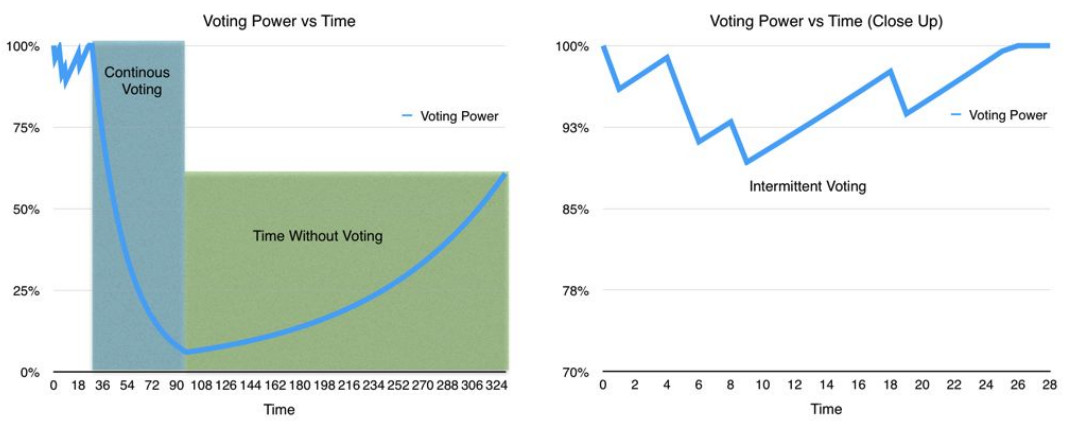
\includegraphics[width=\textwidth]{fig/fig1}
\end{center}

El gráfico de arriba muestra cómo el poder de voto de un usuario decrece cada vez que vota y luego se regenera a medida que pasa el tiempo sin votar. Estos gráficos usan una unidad nominal de tiempo y podría ser hecho a escala de cualquier tasa de voto. Nótese que el poder de voto cae rapidamente durante períodos de votación contínua, y luego se recupera lentamente. El poder de voto es multiplicado por los \textit{tokens} invertidos de un usuario para determinar la parte que debería ser colocada en el pool de pagos para determinado ítem.

\subsubsection{Pagos retrasados}

Para prevenir abusos a futuro, todos los pagos son retrasados por un promedio ponderado de 24 horas a partir del momento en que cada voto fue emitido. Esto asegura que grandes poseedores no puede atinar pagos votando al menos un segundo antes que otros votantes (también conocidos como "cangrejos") tengan la oportunidad de rechazar potenciales abusos. Una vez que se realiza el pago al usuario, el conteo de votos es restaurado a 0. Si vienen votos luego del pago, el proceso vuelve a comenzar.

\begin{center}
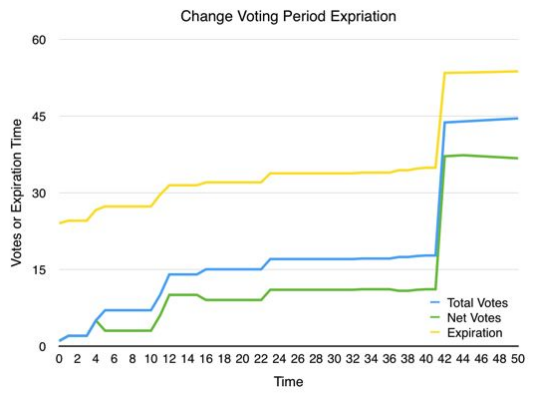
\includegraphics[width=7.5cm]{fig/fig2}
\end{center}

Este gráfico muestra cómo el período de expiración de voto cambia en respuesta a nuevos votos positivos y negativos siendo aplicados. Nuevos votos extienden el período de pago en proporción a cuán grande son relativos a todos los votos que se han sucedido anteriormente. Se puede ver cerca de la línea de tiempo con valor 40 un gran numero de nuevos votos que extienden el período de votación por 12 horas, los votos menores subsecuentes tienen mucho menos impacto en el período de votación.

\subsubsection{Distribución de pagos}

Una de las metas primordiales del sistema de premios de Steem es producir las mejores discusiones on internet. Cada año el 10\% de la capitalización de mercado de Steem es distribuída a los usuarios que envían, votan y discuten contenido. Como el tamaño de \textit{Bitcoin} ésto podría ser tanto como \$1.75 millones de dólares por día siendo entregados a los contribuyentes.

\begin{center}
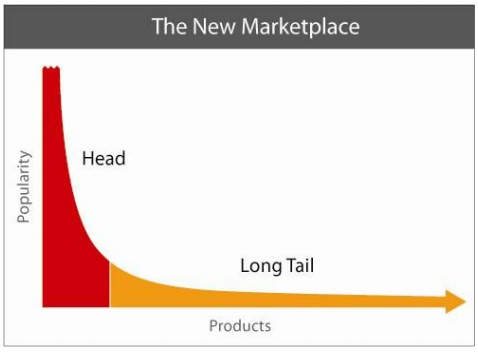
\includegraphics[width=7.5cm]{fig/fig3}
\end{center}

La distribución efectiva dependerá del patrón de votación de los usuarios, pero sospechamos que la amplia mayoría de los premios será distribuída entre el contenido mas popular. Steem prepara los pagos proporcional a \textit{$n^2$} veces el monto de Steem Power votando en un post. En otras palabras, el post p recibirá un pago proporcional a:

\begin{lstlisting}[frame=single]
(votos[p]^2) / suma(votos[0...n]^2)
\end{lstlisting}

La Ley de Zipf\cite{7} es una de esas reglas empíricas que caracterizan muy bien un sorprendente rango de fenómenos del mundo real. Ésta dice que si ordenamos determinada colección grande por tamaño o popularidad, el segundo elemento en la colección medirá aproximadamente la mitad del primero, el tercero un tercio del primero y así sucesivamente. En general, el item en la posición X medirá aproximadamente 1/X del primero.

Tomando la popularidad como una medida de valor tosca, entonces el valor de cada item individual es dado por la Ley de Zipf. Esto es, si tenemos un millón de items, entonces los 100 mas populares contribuirán un tercio del valor total, los próximos 10.000 otro tercio, y los restantes 989.900 el tercio restante. El valor de la coleccion de \textit{n} items es proporcional a \textit{log(n)}.

El impacto de esta distribución de votos y pagos ofrece grandes recompenzas al buen contenido mientras se mantiene el premiado a los pequeños jugadores por el \textit{long-tail} de su contribución.

El efecto económico de ésto es similar a la lotería donde la gente sobreestima su probabilidad de obtener votos y por ende trabaja mas del valor esperado de su premio y por lo tanto maximizan el monto total de trabajo realizado en servicio de la comunidad. El hecho de que todos "ganen algo" juega sobre la misma psicología que suelen usar los casinos para mantener a la gente apostando. Dicho de otra forma, los pequeños premios ayudan a reforzar la idea de que es posible ganar premios mayores.

\paragraph{Recompensas para posts padres}

Una buena discusión requiere posteos hacia adelante y hacia atrás. Cuando usted responde a otro, ellos obtienen un 50\% de cualquier pago que usted obtenga en ese hilo. Esta regla aplica hasta 6 niveles de profundidad. Empezando una gran discusión premia ampliamente al posteador inicial.

Fallar en anidar propiamente sus posts en la discusión es una buena forma de ser votado para abajo.

Esta estructura de incentivo motiva a la gente a contribuír de forma que motiva a otros a involucrarse. Alienta a las personas a hacer buenas preguntas para que otros puedan proveer respuestas valiosas.

\subsubsection{Pagos}

Cuando un post recibe un pago, éste toma la forma de 50\% de SMD y 50\% de SP. El Steem Power da al usuario un poder aumentado de voto y transacción mientras que el SMD da al usuario un beneficio inmediato en una moneda estable. Como ya hemos analizado en profundidad, tanto el SP como el SMD están diseñados para alentar la posesión a largo plazo en lugar de la venta a corto plazo.

\subsection{Algoritmo de consenso}

El consenso es el proceso por el cual una comunidad llega a un acuerdo no ambiguo y universalmente reconocido sobre una pieza de información. Hay muchos algoritmos desarrollados por la sociedad para alcanzar consenso sobre quién es dueño de qué. Cada gobierno en la tierra es un algoritmo de consenso primitivo con el cual la población acuerda atenerse a cierto conjunto de reglas encapsuladas en una Constitución. los gobiernos establecen cortes, jueces y jurados para interpretar hechos subjetivos y emitir una decisión final. La mayoría de las veces la gente se atiene a estas decisiones incluso si son erróneas.

Los algoritmos utilizados por las criptomonedas proveen una mejor forma para alcanzar consenso. Testimonios criptográficamente firmados por individuos son registrados en un registro público que establece un orden global absoluto de eventos. Una algoritmo computacional determinístico puede procesar este registro para derivar una conclusión universalmente aceptada. En tanto los miembros de una comunidad estén de acuerdo en el algoritmo de proceso, el resultado de dicho algoritmo es autoritario.

La consideración primaria es determinar qué testimonio es permitido para entrear el registro público. Los sistemas deberían ser diseñados para minimizar el potencial para su censura. La censura en el registro público es similar a prevenir que alguien vote en una elección. En ambos casos un individuo tiene su impacto en el consenso global imposibilitado.

\subsubsection{Consenso en Steem}

Conceptualmente, el algoritmo de consenso adoptado por Steem es similar al algoritmo de consenso adoptado por compañías de todo el mundo. Gente con interés invertido en el valor futuro de Steem, vota para elegir individuos responsables de incluír testimonios en el registro público. El peso del voto es determinado proporcionalmente al interés invertido de cada individuo.

En el mundo de las criptomonedas, se refiere comunmente al registro público como \textit{blockchain}. Un block o bloque es un grupo de transacciones firmadas (testimonios).

En Steem, la producción de bloques es realizada en rondas. En cada ronda se seleccionan 21 testigos para crear y firmar bloques de transacciones. Diecinueve (19) de éstos testigos son seleccionados para aprobar las votaciones, uno es seleccionado por una prueba-de-trabajo computacional (\textit{Proof of Work}), y un puesto es compartido por tiempo por cada testigo que no logró entrar en el top 19 proporcional de mas votados. Los 21 testigos activos son mezclados en cada ronda para prevenir que cualquiera de los testigos ignore constantemente bloques producidos por el mismo testigo ubicado anteriormente en ese puesto.

Este proceso está diseñado para proveer la mejor confiabilidad mientras se asegura que todos tengan potencial para participar en la producción de bloques independientemente de si son suficientemente populares para ser votados dentro de la lista de los 19 testigos principales elegidos: pacientemente esperan en línea con todos los demás que no estén entre los 19 principales, compran suficiente poder computacional para resolver una prueba de trabajo (\textit{Proof of Work}) mas rápido que otros, o compran mas SP para mejorar su poder de voto. Generalmente hablando, aplicar censura es una buena forma de elegir testigos para perder su trabajo y por lo tanto, es improbable que sea un problema real en la red de Steem.

Debido a que los testigos activos son conocidos de antemano, Steem puede acomodar los testigos para producir bloques cada 3 segundos. Los testigos sincronizan sus producción de bloques a través del protocolo NTP. Una variante de este algoritmo ha sido utilizada por la red \textit{BitShares} por alrrededor de una año donde ha demostrado ser confiable.

\subsubsection{Minando en Steem}

Los \textit{blockchains} de prueba de trabajo (\textit{PoW }ó \textit{Proof of Work}) tradicionales combinan la producción de bloques con la solución de una prueba de trabajo. Debido a que el proceso de resolver una prueba de trabajo toma una cantidad impredecible de tiempo, el tiempo de producción de bloques resulta también indeterminado. Steem apunta a tener una producción confiable y consistente cada 3 segundos casi sin potencial de forks o desvíos.

Para lograr ésto, Steem separa la producción de bloques de la solución de pruebas de trabajo. Cuando un minero resuelve una prueba de trabajo para Steem, éste emite una transacción que contiene el trabajo o resultado. El próximo testigo programado lo incluye entonces en el \textit{blockchain}. Cuando la transacción es efectivamente incluída el minero es añadido a la cola de mineros programados para producir bloques. Cada ronda un minero salta de la cola y es incluído en el conjuto activo de testigos. El minero obtiene el pago cuando éstos producen un bloque en el tiempo que tienen programado.

La dificultad de la prueba de trabajo se duplica cada vez que el largo de la cola crece por 4. Debido a que un minero sale de la cola a cada ronda, y cada ronda toma 21 * 3 = 63 segundos, la dificultad automáticamente se divide si no se resuelve una prueba de trabajo en no más de 21 * 3 * 4 = 252 segundos.

\paragraph{Premios de minado requieren Steem Power}

Luego del primer mes, a los minadores de Steem se les paga en Steem Power (SP). El Steem Power es liquidado a través de un proceso de dos años de \textit{Powering Down}. Esto significa que los mineros deben esperar un buen tiempo, seguramente varios meses, antes de que suficientes premios de minado hayan sido desactivados (\textit{Powered Down}) para permitirles recuperar el costo de electricidad y recursos computacionales. El proceso de \textit{Powering Down} desalienta la creación de pool de minado porque el operador del pool debería tener que repartir los pagos entre años.

El efecto de pagar los premios de minado en SP es la prevención de la utilización del precio diario por parte de los mineros para determinar la ganancia del proceso de minado. Pocos estarán de acuerdo en cuál será el precio en el futuro. Esto quiere decir que la dificultad será determinada por aquellos que depositen mayor estima en el valor a futuro. Los mineros sin un interés en la plataforma a largo plazo serán desalentados de competir. Finalmente se logra que las procedencias de minar sean menos tendientes a ser extraídas del mercado debido a que éstas serán acumuladas por los creyentes de la plataforma a largo plazo.

\paragraph{Algoritmo de minado}

El algoritmo de minado adoptado por Steem requiere que el minero tenga acceso a la clave privada de la cuenta que recibirá los premios. Este requerimiento tiene varias consecuencias importandes. Primero alienta la optimización de los algoritmos de verificación de la firma de curva elíptica requerida por Steem. Segundo, hace más desafiante la instalación de \textit{pools} de minado porque el operador del mismo debería compartir el control de la ganancia con mineros "anónimos". Tercero, dificulta el uso de botnets al hacer que operador necesite distribuír su llave privada a todas las máquinas comprometidas.

El siguiente pseudocódigo describe cómo se calcula el valor del hash de la prueba de trabajo (\textit{Proof of Work}):

\begin{lstlisting}[frame=single]
Let H = Head Block ID
Let H2 = SHA256(H+NONCE)
Let PRI = Producer Private Key
Let PUB = Producer Public Key
Let S = SIGN(PRI, SHA256( H ) )
Let K = RECOVER_PUBLIC_KEY( H2, S )
Let POW = SHA256( K )
\end{lstlisting}

\paragraph{Resistencia a \textit{Botnets}}

Muchas monedas basadas en prueba de trabajo terminan siendo minadas por botnets. Una \textit{botnet} es una colección de miles o millones de máquinas que han sido comprometidas por intrusos informáticos. Estos intrusos roban los recursos computacionales y eléctricos de dichas máquinas comprometidas para minar \textit{tokens} de criptomoneda.

Steem posee varias propiedades que previenen que éstos ladrones computacionales obtengan beneficios. Los operadores de las \textit{botnets} son "empresas" que buscan lucro y típicamente venden sus recursos robados al mayor postor. Esto significa que aquellos que utilizan una \textit{botnet} pagan el poder computacional de la misma forma que lo hace alguien usando el servicio EC2 de Amazon. El requerimiento para impulsar Steem significa que el capital gastado en comprar recursos de la \textit{botnet} estarán atados por un período durante el cual el operador se expone a la volatilidad de los precios.

Otra forma en que se previene que los operadores de las \textit{botnets} obtengan ganancias es la necesidad de que el mismo deba distribuír la llave privada a todas las máquinas comprometidas. Si al menos una de éstas computadoras es descubierta, el operador podría perder las monedas ganadas por toda la botnet.

La última mitigación es la dependencia en la latencia. La mayoría de las \textit{botnets} comprometen computadoras con una conexión a internet pobre, éstas conexiones lentas reducen drásticamente la efectividad del recurso computacional.

Debería ser mas conveniente y menos riesgoso para los operadores de \textit{botnets} usar estos recursos para otras actividades que no sean minar STEEM.

\paragraph{Resistencia a grupos o \textit{pools} de minado}

Los minadores tienen un total de 3 segundos para recibir un bloque, resolver la prueba de trabajo, y obtener la transacción al siguiente productor de bloque. Gran parte de este tiempo se irá en la latencia de la red, lo que implica que es crítico para los mineros poseer buena conexión a la red para lograr un uso efectivo de sus recursos computacionales.

Debido al constante cambio del bloque de cabecera y la latencia de la red, reenviar una plantilla para minar un bloque específico a los participantes del pool o grupo de minado agrega latencia adicional y reduce significativamente la eficiencia del minado en grupo (\textit{pool mining}).

\subsubsection{Eliminando comisiones de transacción}

Steem va más allá para beneficiar a quienes contribuyen a la red. Sería contraproducente dar la espalda y cobrar a los usuarios cada vez que intentan interactuar con la comunidad.

La tecnología \textit{blockchain} actualmente depende de comisiones de transacción para prevenir \textit{spam}. Estas comisiones sufren de todos los problemas conocidos con las microtransacciones y previenen que los \textit{blockchains} sean usados para transacciones de bajo costo. Las aplicaciones verdaderamente descentralizadas deben ofrecer a los usuarios el atractivo de transacciones gratuitas si se desea competir ante sus alternativas centralizadas. Este documento explica el método utilizado por Steem para eliminar la necesidad de comisiones y por ende habilitar un amplio rango de aplicaciones anteriormente inviables de manera descentralizada.

\paragraph{El problema de las comisiones}

Los \textit{blockchains} son redes descentralizadas donde todas las transacciones son emitidas a todos los pares (\textit{peers}). Cada tanto se produce un bloque que incluye alguna o todas las transacciones pendientes. Todos los \textit{blockchains} deben encontrar una solución para prevenir que usuarios maliciosos consuman todo o gran parte de la capacidad disponible de la red con transacciones sin valor o inútiles. Estas transacciones sin valor evitan que transacciones valiosas y útiles sean procesadas en detrimento de la red.

La solución adoptada por la mayoría de los \textit{blockchains} hasta ahora es cargar una comisión mínima de transacción. Una comisión con un costo de unos pocos centavos es suficiente para lograr que atacar la red no sea redituable e incluso costoso. Mientras ésta solución resuelve el problema del \textit{spam}, introduce nuevos problemas. Imagine resolver el problema del \textit{spam} en \textit{emails} introduciendo una pequeña comisión en cada correo enviado; la gente no usaría el correo electrónico.

\subparagraph{Los micropagos no funcionan}

El problema fundamental de cargar comisiones de transacción reside en que los micropagos no funcionan, especialmente por el bajo valor de las acciones de los usuarios. Cuando se carga una comisión en cada transacción, se limitan los tipos de transacciones que una red descentralizada puede procesar. Independientemente de cuán racional sea el argumento para la necesidad de las comisiones, los usuarios aún detestan la experiencia de dejar unos centavos por cada cosa que hacen.

Imagine que los sitios web que usamos a diario cobraran una comisión por cada vez que modificamos nuestras cuentas o cambiamos la contraseña. Los usuarios esperan que ciertas cosas sean gratuitas. Requerir a los usuarios que tomen una decisión sobre que acción merece o no una pequeña comisión crea ansiedad que causa que éstos se retiren.

\begin{displayquote}
Una transacción no puede valer tanto como para requerir una decisión pero vale tan poco que la decisión es automática. Hay cierto monto de ansiedad involucrado en cualquier desición de compra, no importa cuán poco ni el tamaño, y no deriva de la interfaz utilizada o el tiempo requerido, sino del propio acto de decidir. Los micropagos, como todos los pagos, requieren una comparación: \textit{"¿Vale ésta cantidad de X tanto de Y?"}. Hay una costo mental de transacción mínimo creado por este hecho que no se puede optimizar, porque la única transacción que un usuario estaría dispuesto a aprobar sin pensarlo es aquella que no tiene costo, que no es una transacción. – Clay Shirky \cite{8}
\end{displayquote}

En el mundo de los pagos financieros, pequeñas comisiones son aceptables debido a que el valor de la transacción es extremadamente alto en relación a la comisión cobrada, y el comprador ya ha tomado la decisión de comprar. El mundo de aplicaciones potenciales de blockchai es mucho mas grande que simplemente el de pagos financieros e incluye muchas transacciones necesarias para las cuales las comisiones son simplemente inaceptables para los usuarios.

Sistemas como \textit{BitShares}, \textit{NXT}, \textit{Ripple}, \textit{Counterparty} y \textit{Stellar} permiten a los usuarios colocar órdenes de límite en el \textit{blockchain} y todos cobran a los usuarios una pequeña comisión para realizar esta acción. Luego si el usuario desea cancelar su orden, se le cobra otra comisión. Sistemas como \textit{Ethereum} llevan los micropagos a un nivel completamente nuevo: cobrar por cálculo. Todos estos sistemas luchan para atraer nuevos usuarios \textit{mainstream} por la misma razón por la que un motor de búsqueda se esforzaría para atraer nuevos usuarios desde google si cobrara una pequeña comisión por cada búsqueda. No importa cuan bueno sea el servicio, la gente espera que ciertas cosas sean gratuitas. Esto es cierto incluso si un usuario finalmente termina pagando más en una estructura diferente.

\subparagraph{Las comisiones son barreras para el acceso}

Cualquier comisión crea una barrera de entrada a los nuevos usuarios. Antes que alguien pueda experimentar con \textit{Ethereum} debe adquirir \textit{tokens} de \textit{ETH}. Cualquiera que desee desarrollar una aplicación descentralizada en \textit{Ethereum} debe trasladar el costo a sus clientes. Comprar una criptomoneda no es una tarea fácil y raramente tiene sentido por montos menores a \$10. Esto quiere decir que los usuarios nuevos queriendo probar una nueva aplicación descentralizada debe primero ser convencido de empezar con \$10.

\subparagraph{Cambiando las comisiones}

Con el tiempo una red debe ajustar las comisiones. Esto puede suceder tanto por un incremento en el valor del token o al aumento en la capacidad. Los usuarios prefieren comisiones predecibles y servicio garantizado. Aún siendo posible ajustar dinámicamente las comisiones en tiempos de mucho uso, el resultado es una pobre experiencia de usuario.

\subparagraph{Ataques de identidad o Ataques Sybil (\textit{Sybil attacks})}

Los sitios web centralizados previenen el \textit{spam} limitando la frecuencia o alguna forma de verificación de identidad. Incluso algo tan simple como un \textit{CAPTCHA}\cite{9} es suficiente para limitar la creación de cuentas falsas. Si alguien abusa de su cuenta, los sitios web centralizados tienen la libertad de bloquear la cuenta.

En un sistema descentralziado no hay forma directa de prohibir usuarios ni un proveedor centralizado que pueda alojar un \textit{CAPTCHA} para imponer un límite de frecuencia de creación de cuentas. De hecho, la falta de habilidad para censurar usuarios es un de los principales puntos atractivos de la tecnología del \textit{blockchain}.

Reserva completa vs. reserva fraccionada

Veamos el \textit{blockchain} como un Proveedor de Servicio de Internet (\textit{ISP}) cooperativo que posee todos los cables en pueblo y tiene un ancho de banda máximo que puede proveer en cualquier momento. La gente viviendo en el pueblo puede comprar acciones en el \textit{ISP} y a cambio obtienen el derecho de utilizar una porción del ancho de banda disponible.

El \textit{ISP} tiene dos opciones, correr un sistema de "reserva completa" o uno de "reserva fraccional". Bajo un sistema de reserva completa a cada usuario solo se le permite una fracción del ancho de banda máximo proporcional a sus acciones. Debido a que no todos usan Internet al mismo tiempo, la red del pueblo sería sifnificativamente subutilizada.

En un sistema de reserva fraccional los usuarios individuales podrían utilizar mas ancho de banda del que tienen otorgado en cualquier momento mientras no todos usen Internet en ese mismo tiempo. El problema al operar una reserva fraccionada es que las congestiones ocurren cuando mucha gente desea usar la red al mismo tiempo. El \textit{ISP} necesita una forma de priorizar el ancho de banda durante períodos congestionados. En el caso mas extremo, una red completamente congestionada debe revertirse a un sistema de reserva completa. El desafío es implementar la proporción correcta de reserva fraccional.

\paragraph{Iterando mas allá de los micropagos}

La solución a los problemas de los micropagos es implementar reservas fraccionales dinámicas. Bajo este modelo el \textit{blockchain} automáticamente ajustará la proporción de reserva para la red durante períodos de congestión. El \textit{blockchain} ubicará un objetivo de utilización que deje suficiente margen para oleadas de demanda en cortos plazos. En cualquier momento que se mantengan oleadas de uso el \textit{blockchain} reduce el ancho de banda máximo por acción. Cuando una oleada se acaba y sobra capacidad, el \textit{blockchain} puede lentamente incrementar el ancho de banda por acción.

El ancho de banda utilizado por un usuario individual debería ser medido sobre un período de tiempo apropiadamente largo para permitir que el usuario puede invertir el horario de su uso. Los usuarios tienen a acceder, hacer varias cosas al mismo tiempo, y luego salir. Esto significa que su ancho de banda durante un período de tiempo corto puede parecer mucho mas alto que si es visto sobre un período mas largo. Si la ventana de tiempo se estira demasiado entonces la proporcion de reserva no se ajustará lo suficientemente rápido para responder al incremento a corto plazo, si la ventana es demasiado estrecha entonces agrupar el uso tendrá un impacto muy grande en usuarios normales.

En nuestra estimación debería ser suficiente medir el promedio semanal de ancho de banda de los usuarios. Cada vez que un usuario firma una transacción, ésta es ténida en cuenta en el promedio móvil individual del usuario. En el momento en que el promedio móvil de un usuario excede el límite actual de la red, su transacción es retrasada hasta que su promedio se acomode debajo de ese punto.

\subparagraph{Ejemplo de implementación}

Siendo \textit{B} equivalente al promedio de ancho de banda de un usuario sobre el tiempo T. Siendo W equivalente al número de segundos por semana, y siendo N equivalente al tamaño de la nueva transacción ocurrida S segundos después de T, el \textit{blockchain} puede calcular el nuevo promedio de ancho de banda para un usuario cómo:

\begin{lstlisting}[frame=single]
Bnew = MIN(0,B * (W­S) / W) + N * S / W
Tnew = T + S
\end{lstlisting}

Each user is entitled to an average weekly bandwidth of:

\begin{lstlisting}[frame=single]
Let U = the user’s SP
Let S = the total number of SP
Let R = the current reserve ratio between 1 and Rmax
Let C = the maximum block size capacity set by witnesses
Let L = the total blocks per week
Let M = C * L * R
Allocation = M * U / S
\end{lstlisting}

Se le otorgaría a un usuario un promedio de ancho de banda de M * U / S. Cuando una transacción cause que el promedio individual se posicione sobre éste límite, el usuario no podrá transaccionar hasta que pase el tiempo suficiente para bajar el promedio.

La red puede incrementar la proporción de reserva cuando los bloques sean menos que la mitad de la capacidad obetivo y decrecer cuando sean mas de la mitad. El algoritmo utilizado para ajustar R está diseñado para reaccionar rápidamente para disminuír la proporción de reserva cuando hay un pico de demanda, mientras actúa lentamente para incrementar la proporción de reserva en un período de baja demanda.

La proporción mínima de reserva es 1, y la máxima debería ser calculada para prevenir que pequeños participantes consuman todo el ancho de banda disponible. Si nadie se encuentra utilzando el ancho de banda disponible entonces la proporción de reserva puede crecer hasta que un usuario con sólo 1 satoshi de la moneda pueda transaccionar cada bloque.

\subparagraph{Caso de estudio: \textit{Bitcoin}}

Para entender como funcionaría este algoritmo en \textit{Bitcoin} es necesario estimar un valor razonable para la proporción de reserva, R, basados en el uso actual. Basado en el suministro total de 15 millones BTC y un volumen diario de transacciones de 400.000 BTC \cite{10}, podemos deducir una mínima proporción de 38 por \textit{Bitcoin}. Utilizando las ecuaciones podemos calcular que el ancho de banda seanal (en \textit{bytes}) permitidos por BTC es:

\begin{lstlisting}[frame=single]
Let C = 1MB = 1024*1024
Let L = 1008 (blocks per week)
Let R = 38
Let S = 14000000 BTC (supply minus Satoshi’s unmoving coins)
Let U = 1 BTC
CLR/S = 2869 bytes per week, or about 5 transactions/week per BTC
\end{lstlisting}

Debido que \textit{R = 38} es una cota inferior a la tasa de reserva, CLR/S es una cota en el ancho de banda permitido. Este simple caso de estudio sugiere que un usuario requerirá como mucho 0.20 BTC para transaccionar una vez a la semana. Sin embargo, este es una cota superior vaga obtenida asumiendo que todos los BTC son igualmente móviles. Este no es el caso -- usuarios con docenas o cientos de bitcoins no necesariamente transaccionan docenas o centenas de veces por semana. Las transacciones "restantes" que esos usuarios "deberían" haber realizado incrementarán la tasa de reserva, permitiendo que su ancho de banda sin utilizad sea "reciclado" para usuarios mas pequeños.

Todos los estimados de arriba son cotas superiores conservativas asumiendo que las monedas y uso son distribuídas de una forma relativamente plana. La realidad es que los grandes consumidores, como los \textit{exchanges}, tienen una relación de moneda/uso mucho mayor que los usuarios normales, que a su vez implica que los requerimientos del balance mínimo son mucho menores.

\subparagraph{Impacto de capacidad}

La capacidad del \textit{blockchain} no está necesariamente limitada. Está bien dentro de la capacidad tecnológia de la infraestructura internet incrementar el tamaño de bloque de \textit{Bitcoin} a 10MB lo que en cambio reducirá el balance mínimo requerido por un factor de 10. Mientras \textit{Bitcoin} actualmente soporta aproximadamente 3 transacciones por segundo, implementaciones alternativas pueden permitir mas de 1000 transacciones por segundo. Esto modifica nuestra cota superior a 0.0006 BTC, queriendo decir que una cuenta que contenga 0.0006 BTC tendrá la posibilidad de transaccionar al menos una vez por semana en promedio (y posiblemente muchas mas veces porque estamos lidiando con una cota superior mas permisiva).

\subparagraph{Número máximo de usuarios únicos}

Podemos utilizar una matemática similar para calcular el número máximo de usuarios únicos que la red puede permitir transaccionar una vez por semana como: B * W / T. \textit{T} representa el promedio de tamaño de transacción. Esto quiere decir que \textit{Bitcoin} podría soportar alrrededor de 2 millones de usuarios transaccionado una vez por semana asumiendo que cada usuario tuviese el mismo balance.

\subparagraph{Comparación de comisiones}

Si asumimos que un usuario con \$25 dólares en BTC transacciona una vez por semana y paga una comisión de \$0.04 cada vez entonces ellos pagarían mas de \$2 en comisiones por año. Un usuario tendría que ganar una tasa de retorno de 8\% sobre sus \$25 sólo para no salir perdiendo al pagar comisiones. Todo indica que los usuarios van a mantener su dinero en el \textit{blockchain} de todas formas, entonces este usuario con \$25 en BTC ha ahorrado \$2 en el transcurso de un año al adoptar una propuesta de tasa limitada en lugar de una libre de comisiones. Con solo \$175 podrían transaccionar todos los días y ahorrar \$14 al año.

\subparagraph{Creación de cuenta}

El sistema de Steem, basado en cuentas de con balances públicamente conocidos simplifica la implementación del algoritmo de limitación de tasa basado en el ancho de banda. Cualquier cuenta con un balance por debajo del mínimo requerido para transaccionar una vez por semana no debería poder transaccionar. Esto implica que todas las nuevas cuentas deberían ser cargadas con al menos éste balance mínimo. Esto tambien implica que los usuarios deseando transaccionar en montos menores puedan, mientras mantengan un balance mayor y reutilicen la cuenta.

Es posible para una cuenta con balance bajo creada durante un tiempo de bajo uso volverse inaccesible si el uso de la red se dispara. Los fondos podrían ser recuperados en cualqueir momento transfiriendo un balance mayor a la cuenta.

Con el fin de mantener una experiencia de usuario razonable con un mínimo de cuentas colgadas, todas las nuevas cuentas debe comenzar con un balance 10 veces el mínimo requerido para transaccionar por semana. De esta forma si la demanda se incrementa por un factor de 10, la cuenta continuará utilizable.

Cualquier balance de cuenta inicial debería tener que venir del usuario creando la cuenta y no de la creación de token debido al peligro de ataques de identidad (\textit{Sybil attacks})

\subparagraph{Justificando balances mínimos}

El concepto de forzar a los usuarios a mantener un balance mínimo fluye naturalmente del valor de un usuario\cite{11}. Cualquier corriendo un negocio sabe que cada usuario tiene un valor significativo.

Los negocios gastan entre \$30 y \$200 para adquirir un usuario. A veces pagan usuarios directamente, otras veces pagan por publicidad, e incluso otras veces compañías enteras son adquiridas solo por su base de usuarios. Luego de que una compañía adquiere un usuario generalmente le otorga varios servicios gratuitos para mantenerlos cerca lo suficiente para monetizarlos a través de otros medios.

Ripple usa un balance mínimo \cite{12} que escala al uso de recursos de la cuenta y requiere que nuevas cuentas sean fundadas con al menos éste balance mínimo. Actualmente este balance mínimo es de alrrededor de \$0.15, el cual es mayor al \$0.10 que estimamos que permitiría a alguien transaccionar libremente al menos una vez por semana.

Un \textit{blockchain} puede imponer un valor mínimo por usuario a través del simple proceso de requerir un balance mínimo. Cualquier negocio que desee traer un nuevo cliente al \textit{blockchain} puede precargar esa cuenta con un balance mínimo que le permitiría transaccionar. Requiriendo una comisión relativamente grande (\$1.00) para registrar nuevos usuarios naturalmente forzará a cualquiera que ofrezca cuentas gratis considerar la calidad y singularidad de cada cuenta antes de registrarlas con el \textit{blockchain}.

Mantener un balance mínimo es efectivamente lo mismo que hacer que los usuarios paguen comisiones de transacción con el interés que podrían haber ganado en su balance. El balance mínimo es simplemente el balance requerido para ganar suficiente interes para pagar una comisión en un período de tiempo relativamente corto.

Afortunadamente, el balance mínimo requerido puede ser tan bajo como un dólar y ésto es algo que los usuarios pueden entender y apreciar. El costo de oportunidad de interés perdido no incurre en el costo cognitivo de una microcomisión y es mucho mas aceptable para los usuarios.

El STEEM usado para precargar una cuenta es convertido a Steem Power en la nueva cuenta (ej.: \textit{Powering Up})

\subparagraph{Ajustando relación de reserva}

Limitar la tasa requiere que la red ajuste la tasa de reserva lo suficientemente rápido para mitigar el impacto de un atacante intentado inundar la red. Asumamos que el atacante tiene un gran balance, digamos que el 1\% de los \textit{tokens} disponibles. Si tambien asumimos que la red apunta al 50\% de utilización, entonces el ataque sostenido debería encontrar a este usuario estrangulado al 25\% de la capacidad asumiendo que todos tambien esten utilizando 25\% de la capcidad. Dicho de otra forma, el usuario mas grande nunca debería poder consumir mas del 50\% de la capacidad pretendida salvo que posea mas del 50\% del SP (Steem Power)

Usemos una tasa de reserva inicial de 200x. Debido a las reservas fraccionales, ésto significa que cualquiera que tenga el 1\% de los \textit{tokens} tiene el derecho de demandar transacciones con un total de 2 veces el tamaño máximo de bloque. Para llevar el uso de la red por parte del atacante al 25\%, la tasa de reserva debería caer a 25x. Esto causaría que el balance mínimo requerido para transaccionar una vez por semana crezca a 8 veces el mismo.

El \textit{blockchain} puede establecer una tasa de respuesta que indique cualquier incremento sostenido en el uso debería ser rebajado a la capacidad pretendida dentro de un período de tiempo corto (digamos 30 segundos). Un atacantes intentando hacer \textit{spam} en la red no debería poder afectar el servicio a los usuarios normales por mas de un minuto.

Mientras las reducciones en la tasa de reserva deben contrarestar el abuso ráidamente y de forma no-linear, los incrementos en la tasa de reserva deben ser lentos y lineales. Si la red se ajusta en ambas direcciones en 30 segundos entonces el atacante podría dar pulso a la red. Una inundación de transacciones deberpia ser corregida en 30 segundos y luego tomar una hora para volver a los niviles previos al ataque. Bajo este modelo, el atacante puede inundar la red por 30 segundos por cada hora o menos del 1\% del tiempo.

Debe haber una presión lenta en subida constate sobre la tasa de reserva cuando el uso de la red esté por debajo del 50\% hasta que la red alcance la tasa de reserva máximo. La tasa máxima de reserva determina la apuesta mínima requerida para inundar la red en ráfagas cortas.

Cualquier usuario con menos que TOTAL\_DE\_TOKENS / (2 * TASA\_DE\_RESERVA) no podrá producir suficientes transacciones para llenar ni un sólo bloque. Con una tasa de reserva de 200, significa que cualquier usuarios con menos de 0.25\% de la moneda no puede crear suficientes transacciones para retrasar el servicio de nadie.

\subparagraph{Efectividad relativa a comisiones}

Para comparar la efectividad de la tasa de limitación a comisiones debemos considerar cuánto ambos sistemas reaccionan a la inundación intencional de la red por parte de un atacante. En \textit{Bitcoin}, un atacante con \$10.000 puede afectar el servicio por un día entero llenando cada bloque. El mismo atacante no podría afectar el servicio ni siquiera durante un bloque bajo la propuesta de tasa de limitacion de reserva fraccional dinámica.

Si vamos a un caso mas extremo y asumimos que el atacante posee el 1\% de todas las monedas entonces asumimos un atacante con 60 millones dólares. Tal atacante podría denegar el servicio del \textit{blockchain} de \textit{Bitcoin} por 16 años a no ser que los minadores aumentes las comisiones o la capacidad. Incluso si las comisiones fueren incrementadas a \$15 por transacción, el atacantes podría aún continuar afectando la red por 16 dias.

Bajo el enfoque de limitación de tasa, alguien que posea el 1\% de todas las monedas con intenciones de inundar la red lograría su objetivo por menos de 30 segundos.

\subparagraph{Renta vs. Compra vs. Tiempo compartido}

Cuando alguien es dueño de una casa espera el derecho de uso de la misma de forma gratuita. Si un frupo de gente compra una casa en conjunto entonces ellos pueden pretender el derecho de usarla proporcionalmente al porcentaje que les corresponda de la casa. Un \textit{blockchain} basado en comisiones es como rentar la casa a sus propios dueños, donde limitar la tasa es como dividirse el tiempo de uso entre los propietarios.

Si una casa es propiedad de múltiples personas, ellos deben decidir como desean compartir la casa. Alguien que tenga el 50\% de la propiedad pero sólo la utiliza un fin de semana por año podría esperar que los individuos le paguen por el tiempo sin usarla. Esta es la idea de un sistema basado en comisiones.

Por otro lado, alguien que posea el 50\% de la casa está especulando que la demanda por la casa aumente en el futuro y ellos podrán vender su parte por más. Cualquier dueño que posea mas de la casa de lo que utiliza se convierte en un especulador de bienes raíces. Con esta idea en lugar de recolectar renta, recolecta apreciación.

El valor de una acción procede de cuanto tiempo tiempo puede potencialmente otorgar a su propietario. Poseer el 1\% de una casa y obtener un fin de semana por año es el valor mas bajo de una acción. Sin embargo, si la mitad de los propietarios nunca utilizan su fin de semana, entonces el valor por tiempo compartido aumenta a 2 fines de semana por año. Si aquellos usuarios inactivos optan por rentar su tiempo sin uso, entonces éste baja nuevamente a 1 fin de semana por año. Si esos tiempos sin usar fuesen vendidos a gente que los usara entonces el valor del tiempo compartido caería un 50\%. A menos que la renta recolectada sea mayor que la caída del valor de las acciones, los dueños del tiempo compartido estarán cometiendo un error de cálculo económico.

Usando esta racional podemos asumir que un sistema basado en comisiones será mas caro para sus usuarios o ser menos redituable para sus propietarios colectivos. Un propietario individual pequeño puede obtener ganancias al rentar su pequeña porción de tiempo, pero solo a expensa de todos los demás dueños. En efecto, el costo del decreciente valor del tiempo compartido es repartido entre todos los propietarios donde las ganancias son centralizadas en el dueño singular que decidió rentar su parte.

Podemos concluír de ésto que un \textit{blockchain} es mejor servido si no se usa ninguna comisión. Si una comisión de uso fuese cobrada como una alternativa de tasa limitante, entonces debería ser equivalente a comprar el tiempo compartido suficiente y disponerse a mantenerlo el tiempo suficiente para ganar el derecho a usarlo una sola vez.

Dicho de otra forma, una comisión de transacción debería equivaler al balance mínimo de cuenta necesario para transaccionar una vez por semana y debería ser recargado al final de la semana. Asumamos que el mínimo balance de cuenta es \$1 y permite a alguien transaccionar una vez por semana. Si alguien con un balance de \$1 desea concretar 5 transacciones de una sola vez, tendrá que incrementar su balance a \$5 por semana tanto antes o después de sus transacciones.

En teoría un mercado podría formarse donde los usuarios pueden conseguir la inversión necesaria. En la práctica es mas eficiente para los usuarios simplemente comprar y vender el tiempo compartido necesario para alcanzar su tasa de utilización deseada. En otras palabras, el costo de negociar micropréstamos es mayor que el costo de mantener un balance apto para el máximo uso semanal.

La limitación de tasa descentralizada puede habilitar nuevos tipos de aplicaciones descentralizadas que no eran viables cuando todos los usos de la aplicación requerían un micropago. Este nuevo modelo da a los desarrolladores de aplicaciones la habilidad de decidir si y cuando cobrar a sus usuarios por las transacciones.

\paragraph{Performance y escalabilidad}

La red Steem está construpida sobre \textit{Graphene}, la misma tecnología que empodera \textit{BitShares}. \textit{Graphene} ha sido públicamente demostrado sustentando mas de 1000 transacciones por segundo en una red de pruebas distribuída. \textit{Graphene} puede fácilmente escalar a 10.000 o mas transacciones por segundo con mejoras relativamente directas a la capacidad de servidores y protocolos de comunicación.

\subparagraph{Escala Reddit}

Steem puede manejar una base de usuarios mas grande que Reddit. En 2015 los 8,7 millones de usuarios generaron un promedio de 23 comentarios por segundo \cite{13}, con un promedio de 83 comentarios anuales por usuario. Hubieron 73 millones de posts de primer nivel, para un promedio de 2 nuevos posts por segundo. 7 mil millones de votos positivos creando un promedio de velocidad de 220 votos por segundo. Dicho todo ésto, si Reddit estuviese operando en un \textit{blockchain} requerirpia un promedio de 250 transacciones por segundo.

Para lograr esta rendimiento de líder de la industria, Steem ha juntado lecciones aprendidas del \textit{LMAX Exchange}\cite{14}, que puede procesar 6 millones de transacciones por segundo. Entre estas lecciones se encuentras los sigueintes puntos clave:

\begin{enumerate}
\item Mantener todo en memoria.
\item Mantener el núcleo de la logica de negocio en un sólo hilo.
\item Mantener las operaciones criptográficas (hashes y firmas) fuera de la lógica del núcleo de negocio.
\item Dividir la validación en comprobaciones dependientes e independientes del estado.
\item Usar un modelo de datos orientado a objetos.
\end{enumerate}

Al seguir estas simples reglas, Steem puede procesar 10.000 transacciones por segundo sin un esfuerzos significativos en términos de optimización. Mantener todo en memoria es cada vez mas viable dada la reciente introducción de la tecnología \textit{Optane}™ de \textit{Intel} \cite{15}. Debería ser posible para el hardware manejar toda la lógica del negocio asociada con Steem en un sólo hilo con todos los posts mantenidos en memoria para una indexación rápida. Incluso Google mantiene su índice completo de internet en RAM. El uso de la tecnología \textit{blockchain} hace trivial replicar la base de datos en varias máquinas para prevenir la pérdida de datos. A medida que la tecnología \textit{Optane}™ avance, el RAM se volverá aún mas veloz mientras se gana persistencia. En otras palabras, Steem está diseñado para la arquitectura del futuro y diseñado para escalar.

\paragraph{Asignación y suministro}

La red Steem comienza con una provición de moneda de 0 y coloca STEEM a través de la peurba de trabajo (\textit{Proof of Work}) a una velocidad de aproximadamente 40 STEEM por minuto a los mineros, con un adicional de 40 STEEM por minuto siendo creados para financiar el contenido y fondos para premios de curado (totalizando 80 STEEM por minuto). Entonces la red empieza a premiar a los usuarios que convierten a SP. En este punto, STEEM crece a una velocidad de aproximadamente 800 STEEM por minuto debido a los efectos combinados de los disintos Premios de Contribución sumarizados abajo:

\subparagraph{Premios por contribución}

\begin{itemize}
\item Premios de curado: 1 STEEM por bloque o 3,875\% anual, el que sea mayor.
\item Premios de creación de contenido: 1 STEEM por bloque o 3,875\% anual, el que sea mayor.
\item Premios de producción de bloques: 1 STEEM por bloque o 0,750\% anual, el que sea mayor.
\item Premios por inclusión de \textit{PoW }previos al bloque 864.000: 1 STEEM por bloque (entregados como 21 STEEM por ronda)
\item Premios por inclusión de \textit{PoW }posteriores al bloque 864.000: 0,0476 STEEM por bloque (entregados como 1 STEEM por ronda) o 0.750\% anual, el que sea mayor.
\item Premios por liquidez: 1 STEEM por bloque (entregados como 1200 STEEM por hora) o 0,750\% anual, el que esa mayor.
\end{itemize}

\subparagraph{Premios por poder}

Steem Power premia: Por cada STEEM creado por los premios de arriba, 9 STEEM se dividen entre todos los poseedores de Steem Power.

\subparagraph{Operaciones de SMS}

\begin{itemize}
\item Premios SMD: Un porcentaje del valor del SMD es creado en un set APR por los testigos y abonado en forma de SMD a los poseedores de SMD.
\item Tasa de alimentación siguiendo: El monto de STEEM por el cual el total de SMD en existencia puede ser redimidos cambiarán basados en cambios en el índice de precios. Este cambio es efectivamente destrucción de STEEM (quemado o \textit{burning}) cuando el valor de STEEM (tal como lo midan los indicadores) esté incrementándose, o creación de STEEM cuando el valor de STEEM está declinando.
\end{itemize}

Los límites de porcentaje efectivamente aseguran los incentivos por premios no se vuelvan insignificantemente pequeños con el tiempo, el cual está destinado a prevenir que el sistema experimente el "salto de velocidad" en el patrón de crecimiento de muchos otros \textit{blockchains}, donde un chorro de crecimiento inicial impulsado por los altos incentivos de los participantes tempranos es seguidos por un estancamiento prolongado mientras el contínuo declive de incentivos cae por debajo del nivel necesario para inducir a los nuevos a participar.

El efecto completo de estas constantes de porcentaje en la asignación y suministro es que la tasa de 800 STEEM (aproximadamente) pro minuto se mantiene en efecto por largo tiempo (ej.: unidades de STEEM), pero cae en términos de porcentaje (ej.: 800 STEEM es menor y una fracción menor del suministro total mientras que el suministro total crece y crece). Cuando los variados componentes indivuduales de la tasa de 800 STEEM por minuto alcanzan sus respectivos pisos basados en porcenaje, cada piso detiene la caída en su componente de la tasa. Esto en cambio significa que sobre el largo plazo, la tasa nominal aumentará desde 800 STEEM por minuto al (variable en tiempo, dependiente del suministro) valor necesario para mantener un crecimiento anualizaco constante del 10\% para los Incentivos de Contribución, y un crecimiento anual constante del 100\% para el efecto combinado de los Incentivos de Contribución e Incentivos de Poder. El efecto general es una duplicación del suministro de STEEM a cada año (pero, como se explica en la siguiente sección, si la mayor parte de los usuarios hacen \textit{Power Up}, entonces gran parte de esta duplicación es efecticamente una "división" que no transfiere la propiedad).

La imágen general del suministro es complicada por el efecto de las operaciones de SMD, las que pueden resultar en creación o destrucción a larga escala de STEEM a través del seguimiento de tasa de alimentación y premios SMD, como se explica en la sección SMD. Otros efectos de menor escala tambien existen, incluyendo incentivos sin reclamar (ej.: premios de bloque por bloques perdidos), ruido debido a la suerte del minador en la producción de prueba de trabajo, y los efectos de los cambios en la longitud de la cola de minadores debido a un cambio en el total de poder de hash de la red.

\subparagraph{Impacto de Tasa de creación de \textit{tokens}}

A primera vista, un crecimiento anual del 100\% en el suministro de STEEM puede parecer hiper inflacionario y no sustentable. Aquéllos que siguen la Teoria de Cantidad de Dinero \cite{16} pueden incluso llegar a la conclusión de que el valor de STEEM debe caer aproximadamente un 5,6\% por mes. Nosotros sabemos por incontables ejemplos del mundo real que la cantidad de dinero no tiene un impacto directo inmediato en su valor, a pesar de que sin duda juega un rol.

Debido a que el 90\% de todo el STEEM creado es redistribuído de vuelta a los poseedores de SP, el resultado es similar a tener una división de 2:1 cada año en lugar de una verdadera inflación. La tasa total de expendido utilizada para premiar a quienes contribuyen es de alrrededor del 10\% de la capitalización del mercado por año, una tasa bien por debajo de la que sostuvo \textit{Bitcoin} durante los primeros 7 años luego de su lanzamiento.

Crear nuevo STEEM para pagar un incentivo a un usuario o grupo particular tiene un efecto negativo sobre todos los demás balances de usuarios en términos de su porcentaje del sumnistro de STEEM. Si exactamente el 90\% del suministro de STEEM es mantenido en SP, el efecto negativo en los balances de los poseedores de SP es balanceado exactamente por el efecto positivo de los incentivos de poder (\textit{Power Incentives}); Los poseedores de SP obtienen mas STEEM (en términos nominales) pero su porcentaje de la cadena (en términos de fracción del suministro total) se mantiene sin cambios. Si menos (mas) del 90\% del suministro de STEEM es mantenido como SP, ambos efectos aún apuntan en direcciones opuestas, pero el efecto positivo (negativo) se vuelve mayor y la suma de ambos efectos tenderá a tirar el balance de SP hacia el 90\%. Este "tironeo" no implica que el valor del SP debe sostenerse en 90\% sobre el largo plazo, porque los receptores del incentivo pondrán (y en algunos casos deberán) sus STEEM en SP, lo que significa que el "tironeo" hacia el 90\% no es la única fuerza que aplica sobre el porcentaje del suministro de STEEM mantenido como SP.

Desde agosto de 2008 hacia enero de 2009 el suministro de dinero Estadounidense creció desde \$871.000 Millones \cite{17} a \$1.737.000 Millones, a un ritmo de mas del 100\% anual y luego continuó creciendo aproximadamente a un 20\% anual por los siguientes 6 años. Dicho ésto, el suministro de dinero en EEUU ha crecido 4,59x durante menos de 7 años. En el mismo tiempo, el valor del dólar relativo a los bienes y servicios ha caído menos del 10\% de acuerdo a los índices de precios del gobierno \cite{18}. Este ejemplo del mundo real demuestra que el suministro es sólo un componente del precio.

El precio de un \textit{commodity} digital, como STEEM, es conducido tanto por el suministro y la demanda. Si nuevo STEEM es distribuído a aquellos que sostienen a largo plazo entonces el crecimiento en el suministro es desfazado por la correspondiente demanda de sostener. El impacto de este cambio en el suministro es pospuesto hasta una fecha a futuro cuando el poseedor a largo plazo decida vender. La presión para vender es entonces distribuída sobre 2 años.

Cuando un poseedor a largo plazo decida salir, el suministro de STEEM en el mercado se incrementará y empujará el precio hacia abajo. Esta presión es contrarresetada cuando un nuevo poseedor a largo plazo decide comprar STEEM y convertilo de nuevo a SP. Podemos por lo tanto concluír que el precio será mayormente impactado por un cambio en la demanda de sostener STEEM a largo plazo.

Del incremento anual de 100\% en el suministro virtual de STEEM, el 5\% del mismo es en forma de \textit{Steem Dollars} (SMD). SMD representa un compromiso de crear un dolar de STEEM en el futuro y no impacta en el monto de STEEM en el mercado actual. El cambio en la tasa deuda/propiedad puede impactar en el valor percivido del STEEM, pero no se asocia directamente a una caída en el valor de STEEM. Si el valor de Steem aumenta en el tiempo, entonces el monto de STEEM que puede ser creado en el futuro será menor y la "inflación" correspondiente finalmente nunca sucedió.

Dicho ésto, el "gasto" total de Steem es para financiar los montos de premios de contenido, curado, minado, y liquidez a 10\% APR o 1,2\% por mes. La misma transferencia de riquezas podría ser implementada sin ningún cambio en el suministro de STEEM a través de la implementación de una tasa de interés negativo en el STEEM líquido de alrrededor del 10\% mensual. Dicho de otra forma, podría ser implementado cargando una comisión del 3\% (similar a las tarjetas de crédito) en cada transacción y teniendo un 1\% de todo el STEEM transferido a diario. La red de \textit{Bitcoin} transfiere\cite{19} 400.000 BTC de 15,5 Millones (o 2,5\% diario).

El propósito del STEEM líquido es facilitar cambios en la propiedad entre los poseedores a largo plazo. Este es un cambio en la propiedad que la red "grava" para financiar el crecimiento. Esta gravámen a la transferencia puede ser evitado casi por completo por una venta automática de STEEM por SMD semanal cuando la red convierte SP nuevamente a STEEM. El tiempo total gastado en sostener STEEM será tan pequeño que cualquier impacto de cambiar el suministro de STEEM será insignificante comparado a la volatilidad y otras comisiones del mercado.

\subparagraph{Impacto de tasa de creación de \textit{tokens} mayor al noventa porciento}

Al 1ro de mayo de 2016, mas del 98,49\% de todo el STEEM ha sido convertido a SP. Esto demuestra que la demanda a poseer a largo plazo es dominante. En este entorno tanto el STEEM líquido como el SP son diluídos para financiar premios.

Durante los primeros 2 años de vida de la red de \textit{Bitcoin}, se sostuvo una tasa de inflación anual \cite{20} sobre el 100\%. Durante los primeros 5 años estaba sobre el 30\%, y por los primeros 8 años se encontraba sobre el 10\%. De acuerdo a la herramienta para estimar inflación a futuro incluída en el código de fuente de Steem, Steem por contraste logrará una tasa instantánea anual de aproximadamente el 12\% luego de solo 1 año (sin incluír los efectos de las operaciones de SMD)

\subparagraph{Sistema contable}

El incremento en el suministro de STEEM es mayormente un artefacto contable creado por el deseo de evitar la carga de tasas de interpés negativo sobre el STEEM líquido. Las tasas de interés negativo complicarían la vida a los \textit{exchanges} quienes tendrían que ajustar los balances de usuarios para tener en cuenta la tasa negativa de retorno de STEEM depositado. Espejando exactamente la lógica del \textit{blockchain} sería propenso a errores y complicaría la integración y adopción. Por lo tanto, STEEM ha elegido nunca cobrar la cuenta a nadie, pero en su lugar incrementar el suministro. Esto logra un resultado económico similar sin forzar a todos a aceptar depósitos de STEEM para implementar tass de interés negativo en su registro interno.

Un efecto colateral de incrementar el suministro es que la red requerirá niveles constantes de incremento en la precisión de su contabilidad. En promedio el número de bits requeridos para representar una cuenta típica crecerá en un 1.3 anual. Solo tomará 10 años hasta que los números involucrados ya no encajen dentro de la precisión de 53 bits soportada por JavaScript o la precisión de 64 bits soportada por los CPU. Sobre el tiempo la magnitud de los números involucrados crece mas allá de la escala y comprensión humana; incluso, los bits menos significativos tienen tan poco valor económico que los vuelve insignificantes.

Con el fin de compensar el constante incremento de precisión, la red STEEM ejecuta una "división reversa" de 10:1 cada 32.000.000 bloques (aproximadamente 3 años). En este punto en el tiempo todos los balances de STEEM son divididos por 10 y todos los precios se multiplican por 10. Los \textit{exchanges} de criptomoneda tendrán que suspender el intercambio en ese momento y actualizar los balances de cuenta y historial de precios para reflejar la "división reversa" antes de reactivar el intercambio.

Todos los errores de redondeo serán en favor de la red. Cada balance puede perder hasta 0.009 STEEM debido al redondeo, pero este monto de STEEM debería ser económicamente insignificante. Colectivamente todos los poseedores de SP perderán como mucho 0.009 STEEM.

\paragraph{El poder de Steem}

Steem reconoce que el valor de todas las contribuciones de los usuarios (posts y votos) es mayor que la suma de sus partes. Un simple comentario vale casi nada, pero millones de posts curados vale muchos millones (o incluso miles de millones) de dólares. Un solo voto provee poco valor de curado, pero mil millones de votos es un curado efectovo. El contenido sin curado es de valor limitado. Dado todo el contenido de internet menos los enlaces entre éstos, Google lucharía para producir resultados de búsqueda útiles. Son los enlaces entre informaciones que le dan valor significativo.

Por el hecho de que todos se benefician, todos deberían pagar. En otras palabras, ningún usuario individual debería esperar pagar por nada, pero en cambio debería recibir un pago por todo lo que hacen que de valor a Steem. Todo lo que necesitamos hacer es cerciorarnos qué contribuciones de usuario traen un valor de red social y cuales no.

Colectivamente los usuarios de Reddit votan 220 veces por segundo y crean 23 posts por segundo. Reddit está valuado entre \$500 millones \cite{21} y \$4.000 millones \cite{22}, lo que significa que cada uno de los votos y posts valen alrrededor de \$0,06 y \$0,50 asumiento que el valor de Reddit está mayoritariamente dentro del valor de la actividad del año pasado. Uno podría argumentar que la mayor parte del valor de Reddit son las discusiones cercanas al tiempo real que han ocurrido la semana pasada que incrementarían dramáticamente el valor de la nueva actividad. La gente va donde están todos hoy, no donde estuvieron el año pasado.

\subparagraph{Sin micropagos, propina opcional}

Los intentos existentes de integrar una criptomoneda en una plataforma de \textit{social media} se han enfocado en habilitar a los usuarios a pagarse entre sí. Muchos servicios han intentado introducir propinas. La teoría es que si hacemos el acto de dar propina lo suficientemente simple entonces mas gente lo haría. Otros servicios intentan hacer que mas gente pague para promover o empujar el ranking de su contenido. Otros aún intentan construir pequeños mercados de predicción de cuanta propina un artículo recibirá.

Todas estas propuestas recaen en micropagos. Estas difieren solo en quién está haciendo el pago. Todas sufren de falta de compromiso de parte de la gente haciendo los micropagos. En la búsqueda de producción de contenido incentivado los emprendedores han estado tan enfocados en quien deberia pagar que han perdido la noción de la obvia realidad: todos se benefician de las acciones de todos asi que todos deberían pagar o nadie debería pagar, dependiendo en como se mire.

Steem se salta los micropagos por completo porque cuando un usuario vota un post es la comunidad quien paga la cuenta. El mismo monto de dinero será gastado tanto si el usuario vota un post o no y los fondos no vendrán del votante.

La energía mental asociada a tomar una desición económica se vuelve una barrera para la participacion para la mayoría de las personas.

\begin{displayquote}
Ya enfrentamos una multitud de opiciones a diario con respecto a qué acceder en línea en esta era digital de la explosión de información, y cada decisión adicional que debemos hacer simplemente se agrega a la incertidumbre y ansiedad que enfrentamos. Quienes apoyan los micropagos creen que una implementación simplificada puede minimizar la intrusividiad de los micropagos y mejorar la experiencia de usuarios, pero su argumento solo crea doble estándares para el proceso de toma de decisión [2]. Una transacción no puede simultáneamente ser suficientemente valiosa para garantizar una desición y valer tan poco que la desición es automática. \textbf{Las únicas transacciones que los usuarios pueden aprobar sin pensarlo son aquellas que no cuestan nada}, en consecuencia cualquier microtransacción de valor positivo incurrirá en costos mentales a través de su requerimiento de tomar una desición. Además, el costo de transacción mental de hecho crece bajo cierto umbral de valor, un fenómeno que ubica los micropagos en aún mayor desventaja. Por ejemplo, es muy fácil pensar que una copia de los periódicos actuales cuestan \$1, pero los lectores enfrentan mucha mas dificultad y ansiedad en decidir el valor de cada artículo o palabra. Tal dilema solo será replicado y exsacervado si todo el contenido en línea fuese desglosado en sus componentes e individualmente cotizado dentro de un sistema de micropagos.
Micropagos: Un modelo de negocios viable \cite{23}
\end{displayquote}

Bajo Steem, los micropagos son pagados al productor del contenido, pero aquéllos que votan el contenido no pagan. En su lugar, el costo del premio es pagado a través de nuevos \textit{tokens}. Alguien puede ingresar en el sistema, votar para pagarle a alguien, y luego irse del sistema con mas dinero del que tenían cuando comenzaron (asumiendo que la valuación del mercado del sistema de Steem se mantenga constante). En otras palabras, las solución de los micropagos provista por Steem provee una experiencia de usuarios similar a muchos sitios web ampliamente utilizados que tienen contenido moderado.

Además, ¡Steem le paga a la gente para determinar a quién se debería pagar!. Este tipo de pensamiento es revolucionario.

\subparagraph{El valor está en los enlaces}

Internet perdería la basta mayoría de su valor si todos los enlaces entre contenidos fuesen removidos. Es esta relación entre páginas web que permite a Google identificar la mejor receta de tarta de manzanas entre 16 millones de resultados. Sin estos enlaces la única información que Google tendría es la frecuencia de palabras.

Los enlaces pueden tomar varias formas y adaptarse en el tiempo. Cada vez que un usuario vota el contenido en una red social ellos agregan el enlace entre el contenido y ellos mismos. Esto en cambio enlaza al consumidor con el productor a través del contenido. Mientras mas enlaces tenga un red mas valiosa se vuelve la información. Es la conexión intencional y relativa de la información que le da valor.

Una red social puede maximizar el valor extraído de un grupo de contenidos al maximizar la calidad y cantidad de enlaces. Curar contenido es caro y consume tiempo mientras es casi imposible para las computadoras realizar ésto ante la ausencia de enlaces. Steem premia a los usuarios que están entre los primeros en encontrar y enlazar nuevo contenido.

Al incentivar el curado, la red Steem puede usar algoritmos automatizados para extraer la información mas valiosa de un monto masivo de contenido.

\subparagraph{Resolviendo el problema de abordaje de las criptomonedas}

No es fácil meterse en las criptomonedas \cite{24}. Alguien que descubre \textit{Bitcoin} y quiere probarlo rápidamente se da cuenta de que necesitará registrarse a un \textit{exchange} y cargar su cuenta con una tarjeta de crédito o una transferencia bancaria. ¿Qué sería de la tasa de adopción de Facebook si tuviesemos que bifurcar el dinero y dos formas de identificación?

Steem resuelve este problema dándole a cada uno una forma de recibir pagos por hacer tareas simples pero valiosas. Esto ayudará a distribuír ampliamente los \textit{tokens} STEEM. Esto es muy beneficioso porque las criptomonedas tienen un efecto de red (ej.: mas usuarios lo hacen mas útil; para un ejemplo extremo, consideremos que si Satoshi se hubiese quedado el 100\% de \textit{Bitcoin} para sí, \textit{Bitcoin} no valdría nada.)

\subparagraph{Resolviendo el problema de liquidación de las criptomonedas}

Una moneda que es difícil de usar o imposible de vender tiene poco valor. Alguien que viene con \$1,00 en \textit{Bitcoin} descubrirá que cuesta mas de \$1,00 vender ese \textit{Bitcoin}. Tendrá que crear una cuenta en un \textit{exchange}, llevar a cabo una validación KYC, y pagar comisiones. Pequeños montos de criptomoneda son como el cambio chico que la gente no está dispuesta a agacharse a juntar del piso.

Los mercaderes dan a los usuarios un camino para convertir rápidamente su criptmoneda en bienes tangibles y servicios. Estos mercaderes necesitan una moneda vinculada a su unidad de cuenta, normalmente dólares. Aceptar una moneda volátil introduce una carga significativa de contabilidad.

Los mercaderes aceptarán cualquier moneda si ésta incrementa sus ventas. Tener una gran base de usuarios con una moneda estable tal como SMD baja la barrera de entrada para los mercaderes. La presencia de mercaderes mejora el sistema al crear una salida del sistema para los usuarios sin tener que entrar en problemas de utilizar un \textit{exchange}.

Otra forma en que la gente puede liquidar sus pequeños montos de criptomoneda que reciben al participa en la plataforma Steem es a través de dar propina a otros. Esto es como dejar el cambio chico como propina al mesero. Cuando mucha gente deja su pequeña propina ésta se añado a un monto significativo. Usted y el mesero se benefician de la propina.

\subparagraph{Censura}

Steem es una red descentralizada que es operada por mineros en jurisdicciones repartidas en el mundo. Todas las acciones de los usuarios son públicamente grabadas en el \textit{blockchain}, y pueden ser públicamente verificadas. Esto significa que no hay una única entidad que pueda censurar contenido que es valioso para los poseedores de STEEM.

Los sitios web individuales como \textit{steemit.com} puede censurar contenido en su sitio particular, pero el contenido publicado en el \textit{blockchain} es inherentemente tráfico emitido y sitios en todo el mundo pueden continuar haciéndolo disponible.

La libertad de expresión es la fundación del resto de las libertados e infringir la libertad de expresión socava los únicos medios pacíficos de alcanzar consenso: la discusión. Sin discusión libre los votantes no pueden ser completamente informados y votantes desinformados son una mayor amenaza para la sociedad que perder el derecho a votar. La censura es un medio para robar votos a través de la limitación del discurso público. Steem está comprometido a habilitar la libertad de expresión y construír una sociedad libre.

\subparagraph{Resolviendo el descubrimiento orgánico a través de la optmización en motores de búsqueda}

La mayoría de las criptomonedas generan poco valor para aquellos que no usan la red activamente. Steem, por contraste, genera contenido y alienta a los usuarios a compartirlo. Este contenido es indexado por motores de búsqueda y finalmente traerán valor a un gran número de usuarios pasivos. Este tráfico de búsqueda crea publicidad orgánica para la red Steem y hace crecer el efecto de red.

\subparagraph{Viraje hacia la atribución basada en \textit{blockchain}}

Internet representa el medio mas fácil para distribuír información en el mundo. Dicho ésto, puede ser un lugar aterrador para los creadores de contenido que quieran ser dueños de su contenido y lo tienen compartido con la atribución correspondiente. En las plataformas de \textit{social media} actuales, la atribución es algo que puede perderse de la noche a la mañana - un video posteado o una imagen pueden ser replicados y recompartidos sin consentimiento o reconocimiento al creador.

Bajo la \textit{social media} basada en \textit{blockchain}, un creador o autor siempre estaría habilitado para apuntar a un registro público y sello de fecha mostrando una prueba del origen de su contenido. En una circunstancia donde el creador quiera encargarse de quienes hayan compartido el contenido sin permiso o atribución, los registro basados en el \textit{blockchain} proveen una prueba pública de que el contenido fue posteado por un usuario particular en determinado momento. En el futuro, la atribución basada en \textit{blockchain} puede ser reconocida por gobiernos por su autenticidad y podría tener peso en la corte, lo cual daría a los creadores de contenido mayores poderes para controlar su trabajo.

Mientras el servicio de sellado de tiempo puede ser construído en casi cualquier \textit{blockchain}, y muchos esfuerzos existen para armar este tipo de servicios en la red \textit{Bitcoin}, Steem tiene una ventaja muy útil en este aspecto porque los publicadores de conteniod son "ciudadanos de primera clase" -- el \textit{blockchain} de Steem está construído desde cero alrrededor del caso de uso de publicación de contenido, lo que permite a los creadores de contenido tener al \textit{blockchain} validando su contenido en determinado punto en el tiempo simplemente por escribir un post usando las mismas herramientas de creación que usan otros usuarios de Steem.

\subparagraph{Reemplazando la publicidad con recompenzas de contenido basado en \textit{blockchain}}

Bajo la mayoría de modelos de monetización, los creadores de contenido apalancan la publicidad de una forma y otra. Muchos creadores reconocen cuanto la publicidad puede disminuír el valor de su trabajo la consumidor, tambien los creadores muy a menudo deben buscar retornos en su tiempo a través de la monetización. La publicidad representa una espada de doble filo: Con anuncios, un creador puede generar dinero mas fácil. Sin anuncios, la monetización se hace difícil pero el contenido es mas rico.

Los creadores subiendo contenido a depósitos de \textit{social media} que están conectados a Steem pueden monetizar simplemente por tener su trabajo reconocido (o "enlazado") por la comunidad Steem. Los pagos basados en \textit{blockchain} son completamente digitales y no tienen intermediarios. Por lo tanto la monetización por premios de contenido basados en \textit{blockchain} deberían ser mas rápidos y con menos barreras para usar que la monetización por publicidad.

\section{Conclusión}

Steem es un experimento diseñado para hacer frente a los desafíos en las industrias de \textit{social media} y criptomonedas combinando los mejores aspectos de ambas. Steem presenta oportunidades de ganancias a los creadores de contenido y lectores de internet de formas que aún no existían dentro de la industria de \textit{social media}. Dentro de Steem, los individuos reciben ganancias reales en línea que son directamente correlativas a sus contribuciones. Esos premios tendrán un valor de dólar debido a al mercado de descubrimiento de precios y liquidez de Steem, y la gente que sostenga Steem tendrá mas poderes gananciales exclusivos que aquellos que no.

\newpage

%%% Bibliography

\begin{thebibliography}{99}
\raggedright
\bibitem{1}
Reddit’s Cryptocurrency, Forbes, Erika Morphy, Octubre 2014, \url{http://www.forbes.com/sites/erikamorphy/2014/10/01/reddits-cryptocurrency-could-have-many-uses/#4e07b05332b9} 
\bibitem{2}
Sweat Equity, Investopedia, \url{http://www.investopedia.com/terms/s/sweatequity.asp}
\bibitem{3}
Meta-moderacion es un segundo nivel de moderación de comentarios. Los usuarios son invitados a valuar las decisiones de los moderadores para mejorar la moderación. \url{https://en.wikipedia.org/wiki/Meta-moderation_system}
\bibitem{4}
The Impossible Trinity, teoría económica \url{https://en.wikipedia.org/wiki/Impossible_trinity}
\bibitem{5}
Metcalfe’s Law \url{https://en.wikipedia.org/wiki/Metcalfe%27s_law}
\bibitem{6}
The Story of the Crab Bucket, \url{http://guidezone.e-guiding.com/jmstory_crabs.htm}
\bibitem{7}
Zipf’s Law \url{https://en.wikipedia.org/wiki/Zipf%27s_law}
\bibitem{8}
Clay Shirky, The Case Against Micropayments \url{http://www.openp2p.com/pub/a/p2p/2000/12/19/micropayments.html}
\bibitem{9}
reCAPTCHA, Easy on Humans, Hard on Bots \url{https://www.google.com/recaptcha/intro/index.html}
\bibitem{10}
Bitcoin Estimated Transaction Volume \url{https://blockchain.info/charts/estimated-transaction-volume?showD}
\bibitem{11}
Forbes, Tristan Louis, “How Much is a User Worth?” \url{http://www.forbes.com/sites/tristanlouis/2013/08/31/how-much-is-a-us}
\bibitem{12}
Ripple, Account Reserves \url{https://ripple.com/build/reserves/}
\bibitem{13}
Reddit Statistics, Number of Users and Comments per Second \url{http://expandedramblings.com/index.php/reddit-stats/2/}
\bibitem{14}
Martin Fowler, The LMAX Architecture \url{http://martinfowler.com/articles/lmax.html}
\bibitem{15}
Introducing Intel Optane Technology – Bringing 3D XPoint Memory to Storage and Memory Products \url{https://newsroom.intel.com/press-kits/introducing-intel-optane-technology-bringing-3d-xpoint-memo ry-to-storage-and-memory-products/}
\bibitem{16}
Quantity Theory of Money, \url{http://www.investopedia.com/articles/05/010705.asp} 
\bibitem{17} 
United States Money Supply, 2009 \url{https://research.stlouisfed.org/fred2/graph/?s%5B1%5D%5Bid%5D=AMBNS}
\bibitem{18}
CPI Inflation Index, United States Dollar 2008-2016 \url{http://data.bls.gov/cgi-bin/cpicalc.pl?cost1=1&year1=2008&year2=2016}
\bibitem{19}
Bitcoin Transaction Volume \url{https://blockchain.info/charts/estimated-transaction-volume}
\bibitem{20}
Bitcoin Annual Inflation Rate, Bitcoin Talk Forum \url{https://bitcointalk.org/index.php?topic=130619.0}
\bibitem{21}
Reddit Valuaton, Newsweek, 2014 \url{http://www.newsweek.com/investors-think-reddit-worth-500-million-26}
\bibitem{22}
Worth of Web, March 2016 \url{http://www.worthofweb.com/website-value/reddit.com/}
\bibitem{23}
Micropayments: A Viable Business Model \url{http://cs.stanford.edu/people/eroberts/cs181/projects/2010-11/Microp}
\bibitem{24}
Dailydot, Jon Southurt, April 2015 \url{http://www.dailydot.com/opinion/bitcoin-cryptocurrency-adoption-hard}
\end{thebibliography}

\end{document}
